%**************************************************
%TEMPLATE TAKEN FROM: 
%https://seanbone.ch/latex-template-exam-summary/
%**************************************************

% Use extarticle for the smaller font size:
% https://tex.stackexchange.com/questions/5339/how-to-specify-font-size-less-than-10pt-or-more-than-12pt
\documentclass[a3paper, 8pt]{extarticle}

\usepackage[document]{ragged2e}

% Multi-column layout
\usepackage{multicol} \setlength\columnsep{9pt}
\usepackage{graphicx}
\graphicspath{ {./images/} }

\usepackage{xcolor, soul}
\sethlcolor{yellow}


% Manually set page margins
\usepackage[margin=0.5cm, bmargin=0.8cm, landscape]{geometry}

\usepackage{centernot}
%\usepackage[T1]{fontenc}
%\usepackage{lmodern}

\newcommand{\notiff}{%
  \mathrel{{\ooalign{\hidewidth$\not\phantom{"}$\hidewidth\cr$\iff$}}}}

% TO DO
% MORE HEAD SPACES FOR THEOREMS
% Replace graphics from slides with grpahics form Lecture notes
% Margins of pictures
% Name theorems correctly
% Less space after Definition
% Manually set margins on lists
\usepackage{enumitem}
% Change list margins - https://tex.stackexchange.com/questions/10684/vertical-space-in-lists
\setlist{leftmargin = 4mm, nosep, topsep=0pt}

\usepackage{graphbox,graphicx}


% \setlist{noitemsep} to leave space around whole list
%create new list type
\newlist{mylist}{enumerate}{4}

\setlist[itemize]{topsep=0pt, nosep, parsep=0pt, leftmargin=3mm}


%Defining a Definition for proofs and stuf


\usepackage{amsmath}
\usepackage{mathtools}
\usepackage{amssymb}
\usepackage{graphicx}
\usepackage[english]{babel}
\usepackage{blindtext}
\usepackage{amsthm}
\usepackage{gensymb}
\usepackage{parskip}
\usepackage{titlesec}
\usepackage{xcolor}
\usepackage[dvipsnames]{xcolor}

\usepackage{enumitem}

\usepackage[parfill]{parskip}



\titleformat{\section}
[hang]
{\RaggedRight \fontsize{12}{12} \sc}
{\thesection}
{5pt}
{}
[\hrule]

\titleformat{\subsection}
[hang]
{\RaggedRight \fontsize{10}{10} \sc}
{\thesubsection}
{4pt}
{}
[\hrule]

\titleformat{\subsubsection}
[hang]
{\RaggedRight}
{\thesubsubsection}
{4 pt}
{}
[\hrule]

\titleformat{\paragraph}
[hang]
{\RaggedRight \underline}
{}
{}
{}
[\pr]



\titlespacing{\paragraph}{}{2pt}{0pt}

\titlespacing{\subsection}{}{6pt}{4pt}

\titlespacing{\subsubsection}{0pt}{8pt}{4pt}

\titlespacing{\section}{}{10pt}{6pt}

\titlespacing{\theorem}{0pt}{0pt}{0pt}


\usepackage{amsmath}

\usepackage{amsthm}
\newtheorem{theorem}{Theorem}[section]

\newtheorem*{theorem*}{Theorem}

\newtheorem{corollary}{Corollary}[theorem]

\newtheorem{proposition}{Proposition}[section]

\newtheorem*{corollary*}{Corollary}

\newtheorem{lemma}[theorem]{Lemma}

\newtheorem*{definition}{Definition}

\newtheorem*{remark}{Remark}



\title{Compressed exam summary}
\author{Paul Gruenenwald}




\begin{document}

\setlist[itemize]{ topsep=0pt}

% Make formulas more compact
%Better alternative to sections
% 3-column layout

%\fontsize{6pt}{6pt}\selectfont
%\tiny
%\scriptsize
%\renewcommand{\familydefault}{\rmdefault}

\setlength{\abovedisplayskip}{6pt}
\setlength{\belowdisplayskip}{6pt}
\setlength{\abovedisplayshortskip}{5pt}
\setlength{\belowdisplayshortskip}{5pt}


\RaggedRight

\begin{multicols*}{6}
%\paragraph{Sentential Form}
%is any string derivable from the start symbol. Thus, in the derivation of a + a * a , E + T * F and E + F * a and F + a * a are all sentential forms as are E and a + a * a themselves.
%\paragraph{Sentence}
%is a sentential form consisting only of terminals such as a + a * a.
       
\section{ Regular Expressions}
\subsection{Alphabets, Words, Languages}

        \textbf{language} over alphabet $\Sigma$ is a (finite or infinite) set of words over $\Sigma$. $\Sigma{^*}$: Set of all words over $\Sigma$
\subsubsection{Inductive Definition of Strings}
        %The Set $\Sigma{^*}$ of all strings over an alphabet $\Sigma$ can alternatively be defined in an inductive fashion:
        $\epsilon \in \Sigma^*$. If $w \in \Sigma^* \text{ and } \sigma \in \Sigma \text{, then } w\sigma \in \Sigma^*$
       % Among other things, this allows the inductive definition of functions on strings. \\Inductively define the function $\#_a$, which assigns to each string $w$ from $\{a, b\}^*$ the number of appearances of the character $a$ in $w$:
        %\begin{itemize}
        %    \item $\#_a(\epsilon) = 0$
         %   \item $\#_a(w \sigma) =$ \begin{cases}
          %      \#_a(w) + 1 &\text{ if } \sigma = a\\
          %      \#_a(w) &\text{ if } \sigma = b\\
          %  \end{cases}
        %\end{itemize}

        
\subsubsection{Prefixes, Suffixes, Substrings} If \textit{x,y,z} are words and \textit{w=xyz}, then (1) \textit{x} is a \textbf{prefix} of \textit{w}
        (2) \textit{y} is a \textbf{substring} of \textit{w}
        (3) \textit{z} is a \textbf{suffix} of \textit{w}. Note that \textit{x,y,z} can all be empty
        
       % \paragraph{\fontsize{7}{6}\sc Interval Notion for Substrings}
        
        \subsubsection{Simple and complex Alphabets}
        Alphabets can also be sets of words. A language can be seen as an alphabet, where each word is a symbol in the alphabet.
        

%\subsection{Syntax and Semantics}
   \stepcounter{subsection} %\subsubsection{Descriptive Formalism: Demands}
    \stepcounter{subsubsection}
%    Precisely describe the syntax of the language we are interested in. At least three construction elements are needed:
    %\begin{itemize}
      %  \item \textbf{repeat} \textit{b* $\equiv$ "arbitrarily many bs"} corresponds to the language $\{ \epsilon, b, bb, bbb, bbbb, ...\}$       
     %   \item \textbf{concatenate} $ab$
      %  \item \textbf{choose} $b+x$
    %\end{itemize}
    
    \subsubsection{Syntax} 
    Formal structure or \textit{set of rules} defining a model
    
\begin{definition} (Regular Expressions).
    \begin{enumerate}
        \item \begin{enumerate}
            \item[a)] The symbol $\emptyset$ is a regex
            \item[b)] The symbol $\epsilon$ is a regex
            \item[c)] For each $\sigma \in \Sigma, \sigma$ is a regex
        \end{enumerate}
        \item If $\alpha$ and $\beta$ are regex then
        \begin{enumerate}
            \item[a)] $(\alpha \beta)$ is a regex
            \item[b)] $(\alpha + \beta)$ is a regex
        \end{enumerate}
        \item If $\alpha$ is a regex, then $(\alpha^*)$ is a regex.
    \end{enumerate}
\end{definition}
    
    \subsubsection{Semantics} 
    \textit{Meaning} of a model, what it can express. The semantics of regular expressions assign a language $L(\alpha)$ to each RE $\alpha$.
    
    \subsubsection{Operators on Languages}
        %\item Let L be a language, then\\ $L^* = \{u_1 ... u_n | u_1, ... u_n \in L, n \in \mathbb{N}_0\}$\\ e.g $\{ab\}^*= \{\epsilon, ab, abab, ababab, ... \}$
        
        $L_1 \circ L_2 = \{uv \;|\; u \in L_1, v \in L_2\}$\\
    $\{ab\}^* \circ \{ccc\}^* = \{ \epsilon, ab, ccc, abccc, abab, ...\}$
    
    
    \begin{definition} (RegEx: Semantics).\begin{itemize}
        \item $L(\emptyset) = \emptyset$
        \item $L(\epsilon) = \{\epsilon \}$
        \item $L(\sigma) = \{\sigma \}$, for each $\sigma \in \Sigma$
        \item If $\alpha$ and $\beta$ are regular expressions, then: \begin{enumerate}
            \item[] $L((\alpha \beta)) = L(\alpha) \cdot L(\beta)$
            \item[]  $L((\alpha +  \beta)) = L(\alpha) \cup L(\beta)$
        \end{enumerate}
    \end{itemize}
    \end{definition}
    
    \paragraph{Regular Language} a language that can be described by a regex. The \hl{complement of a regular language is also regular}

\subsection{Extended Notation}
 \paragraph{Precedence rules}
 (1) Brackets; (2) *; (3) concatenation; (4) +

\begin{tabular}{l l}
    $[a-z] \equiv a + ... + z$ &  \\
    $\alpha? \equiv\: (\alpha + \epsilon)$ & $\alpha$ \textit{ once or never}\\
    $\alpha^+ \equiv\: \alpha\alpha^*$ & $\alpha$ \textit{ at least once} \\
    $\alpha^n \equiv\: \alpha...\alpha$ & $\alpha$ \textit{ repeated n times} \\
    $\alpha^{\{m,n\}}$ & \textit{min. m, max. n times} \\
    $\Sigma^k$ & \textit{All strings of length } k

\end{tabular}

\subsection{ Equivalences of RegEx}
Two regular expressions are equivalent if they describe the same language. We write $\alpha \equiv \beta$ if $L(\alpha) = L(\beta)$.

\subsubsection{Equivalence Rules} 
    %\paragraph{Theorem 1.1} The following equivalences hold for arbitrary regular expressions $\alpha, \beta, \gamma$:

\begin{tabular}{l l}
  Associativity &$\alpha + (\beta + \gamma) \equiv (\alpha + \beta) + \gamma$\\
     &$\alpha (\beta \gamma) \equiv (\alpha \beta) \gamma$ \vspace{7pt}\\ 
Commutativity &$\alpha + \beta \equiv \beta + \alpha$ \vspace{7pt} \\ 
Neutral elements & $\emptyset + \alpha \equiv \alpha \equiv \alpha + \emptyset$\\
&$\epsilon \alpha \equiv \alpha \equiv \alpha \epsilon$ \vspace{7pt}\\ 
Distributivity & $\alpha(\beta + \gamma) \equiv \alpha \beta + \alpha \gamma$\\
&$\epsilon \alpha \equiv \alpha \equiv \alpha \epsilon$\vspace{7pt} \\
Idempotence & $(\alpha^*)^* \equiv \alpha^*$ \vspace{7pt} \\
Zero element & $\emptyset \alpha \equiv \emptyset \equiv \alpha \emptyset$\\
& $\emptyset^* \equiv \epsilon$
\end{tabular}


\subsubsection{Proofs of Equivalences} 

        
        \textbf{Proof method: Equality of sets} The equality of two sets $M_1, M_2$ is best shown in two steps:
            \begin{itemize}
                \item Show that $M_1 \subseteq M_2$
                \item Show that $M_2 \subseteq M_1$
                \item $\forall w \in M_1$, show that $w \in M_2$
                \item $\forall w \in M_2$, show that $w \in M_1$
            \end{itemize}
        
        Show that $\alpha(\beta+\gamma) \equiv \alpha \beta + \alpha \gamma$. In other words show that $L(\alpha(\beta+\gamma))=L((\alpha \beta + \alpha \gamma)$
        \begin{itemize}
            \item Let $\alpha, \beta, \gamma$ be arbitrary.
            \item Here we only show: $L(\alpha(\beta + \gamma)) \subseteq L(\alpha \beta + \alpha \gamma)$
            \item Let $w$ be an arbitrary string in $L(\alpha(\beta+\gamma)):$
            \begin{itemize}
                \item Then there are $u \in L(\alpha)$ and $v \in L(\beta + \gamma)$ with $w = uv$
                \item Then, $v \in L(\beta)$ or $v \in L(\gamma)$
            \end{itemize}
            We distinguish between two cases:
                \begin{enumerate}
                    \item $v \in L(\beta)$: Since $u \in L(\alpha)$ and $v \in L(\beta), w = uv \in L(\alpha \beta) \implies w \in L(\alpha \beta + \alpha \gamma)$
                    \item $v \in L(\gamma): w = uv \in L(\alpha \gamma) \implies w \in L(\alpha \beta + \alpha \gamma)$
                \end{enumerate} 
            \item The proof of $L(\alpha \beta + \alpha \gamma) \subseteq L(\alpha(\beta+ \gamma))$ proceeds similarly.
        \end{itemize}
    
\subsubsection{Proofs of Non-Equivalences} 
    Find a counter example
 
 %\section{\fontsize{10}{6}\sc Proofs} \vspace{-2pt}\hrule\vspace{10pt}   
    
    %\subsubsection{\fontsize{8}{6}\sc Deductive Proofs} 
    %\vspace{-3pt}
    
    %\subsubsection{\fontsize{8}{6}\sc Reformulating statements} 
    %\vspace{-3pt}
    
    %\subsubsection{\fontsize{8}{6}\sc Proofs by contradiction} 
    %\vspace{-3pt}
    
    %\subsubsection{\fontsize{8}{6}\sc Proofs by Induction} 
    %\vspace{-3pt}
    
\section{Finite Automata} 

\subsection{Deterministic Finite Automata} 

\begin{definition}
    (DFA). \textbf{finite automaton} $\mathcal{A}$ is a quintuple consisting of
    \begin{itemize}
        \item finite set Q of \textbf{states}
        \item an \textbf{input alphabet} $\Sigma$
        \item \textbf{transition function} $\delta: Q \times \Sigma \to Q$
        \item an \textbf{initial state} $s \in Q$
        \item a set $F \subseteq Q$ of \textbf{accepting states}
    \end{itemize}
    We write $\mathcal{A} = (Q;\Sigma, \delta, s, F)$
\end{definition}

\begin{center}
 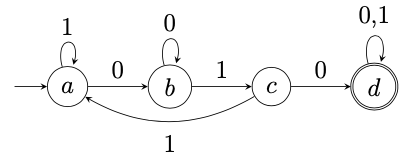
\includegraphics[width=0.7\columnwidth]{images/Screen Shot 2022-11-24 at 12.45.09.png}   
\end{center}


\begin{enumerate}
    \item[] $\mathcal{A}_{010} = (Q_{010}, \{0, 1\}, \delta_{010}, s_{010}, F_{010})$
    \item[] $Q_{010} = \{ a, b, c, d\}$
    \item[] $s_{010} = a$
    \item[] $F_{010} = \{ d \}$
    \item[] $\delta_{010}(a, 0) = b, \delta_{010}(a,1) = a, ...$
\end{enumerate}

\stepcounter{subsubsection}

\subsubsection{Semantics}
\paragraph{Informal Semantics}
\begin{itemize}
    \item Beginning in the initial state, the automaton reads the input character by character
    \item Using the transition function the automaton is able to switch states
    \item The automaton accepts the input if the finishing state is in $F$
\end{itemize}

\paragraph{Formal Semantics}
Assigns to each finite Automaton $\mathcal{A}$ the language $L(\mathcal{A})$
\begin{definition}
    (DFA Semantics).The \textbf{extended transition function} $\delta^*:Q \times \Sigma^* \to Q$ of an automaton $\mathcal{A}$ defined inductively:\begin{itemize}
            \item $\delta^*(q, \epsilon) = q$
            \item $\delta^*(q, u \sigma) = \delta(\delta^*(q,u),\sigma), \text{ for } u \in \Sigma^*, \sigma \in \Sigma$        \end{itemize}

    $\mathcal{A}$ \textbf{accepts} $w \iff \delta^*(s, w) \in F$
        \\ The language \textbf{decided} by $\mathcal{A}: L(\mathcal{A}) = \{w \in \Sigma^* \:|\: \mathcal{A} \text{ accepts }w\}$
\end{definition}

$\delta^* (q,w)$ is the state that $\mathcal{A}$ reaches after reading the string $w$ when starting from state $q$ is
 

\subsection{Nondeterm. Finite Automata} 
We allow multiple transitions for the same symbol thus can not be perfectly reconstructed.
%\subsubsection{NFA Definition}
\stepcounter{subsubsection}
\begin{definition} (NFA) $\mathcal{A}=(Q, \Sigma, \delta, s, F)$ consists of \begin{itemize}
    \item set Q of states
    \item input alphabet $\Sigma$
    \item initial state $s \in Q$
    \item set F of accepting states
    \item a \textbf{transisiton relation} $\delta \subseteq Q \times \Sigma \times Q$
\end{itemize}
\end{definition}
Similar to DFA except transition relation rather than transition function.

We say that the automaton \textbf{accepts} a word $w$ if a computation exists in which $w$ is completely read and an accepting state is reached.
\subsubsection{NFA Semantics}
    \begin{definition}(Run) $\rho$ through an NFA is a sequence of $q_0, \sigma_1, q_1, ... \sigma_n q_n$ where:
    \begin{itemize}
        \item $\forall i \in \{0, ... , n\} : q_i \in Q$
        \item $\forall i \in \{1, ... , n\} : \sigma_i \in \Sigma$
        \item $\forall i \in \{1, ... , n\} : q_{i-1} \overset{ \sigma_i\vspace{0.1pt} \:}{\to} q_i$
    \end{itemize}
    \end{definition}  A run is a sequence of the form \textit{state, symbol, state, ..., symbol, state} with valid relations between the states.

    $p \overset{w}{\to}q$: $\exists$ a run from state $p$ to state $q$

\subsection{NFA with $\epsilon$-Transitions}
These transitions “increase the nondeterminism”, since they add the possibility to change states without reading a symbol.

\subsection{Converting REs into NFAs}
%\begin{itemize}
    %\item  REs can be inductively converted into NFAs
    %\item For $(0 + 1)^*(011 + 001)0$ we obtain these partial automata:
    %\begin{center}
     %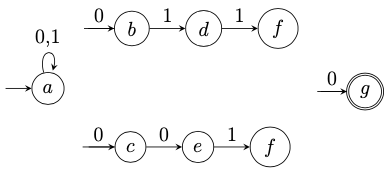
\includegraphics[width=0.8\columnwidth]{images/Screen Shot 2022-11-24 at 12.47.15.png}  
    %\end{center}
    %\item The individual parts can then be pieced together into one automaton:
    %\begin{center}
      %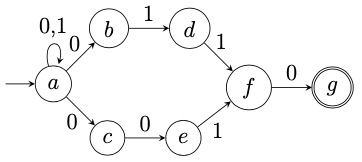
\includegraphics[width=0.7\columnwidth]{images/Screen Shot 2022-11-24 at 12.48.47.png}  
    %\end{center}
    
%\end{itemize}


%We show a stronger statement: $\mathcal{A}$ can be constructed in a way that: \begin{itemize}
    %\item No transitions lead into the initial state
    %\item From the unambiguously defined accepting state no outgoing transitions exist
%\end{itemize}


 \subsubsection{From REs to $\epsilon$-NFAs}
\begin{theorem}
For every RE $\alpha$ $\exists$ an $\epsilon$-NFAs $\mathcal{A}$ such that $L(\alpha) = L(\mathcal{A})$
\end{theorem}
\begin{tabular}{l l}
    $\alpha = \emptyset:$ & \vcenter{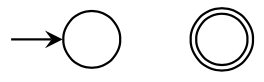
\includegraphics[width=1.5cm]{images/Screen Shot 2022-12-24 at 12.53.41.png}} \\
    $\alpha = \epsilon$: & \vcenter{ 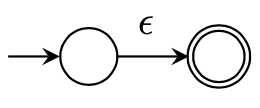
\includegraphics[width=1.5cm]{images/Screen Shot 2022-12-24 at 12.55.15.png}} \\
    $\alpha = \sigma:$ & \vcenter{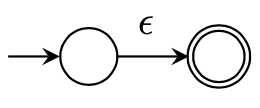
\includegraphics[width=1.5cm]{images/Screen Shot 2022-12-24 at 12.55.15.png}} \\
    $\alpha = \beta \gamma:$ & \vcenter{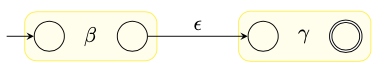
\includegraphics[width= 4cm]{images/Screen Shot 2022-12-24 at 12.46.17.png}} \\
    $\alpha = \beta^*:$ & \vcenter{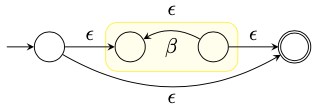
\includegraphics[width=4cm]{images/Screen Shot 2022-12-24 at 12.51.48.png}}\\
    $\alpha = \beta + \gamma:$ & \vcenter{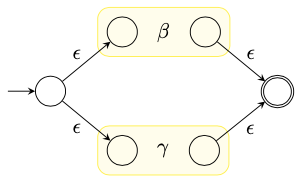
\includegraphics[width=3.5cm]{images/Screen Shot 2022-12-24 at 12.49.27.png}}
\end{tabular}



The individual parts can then be pieced together into one automaton:
    \begin{center}
      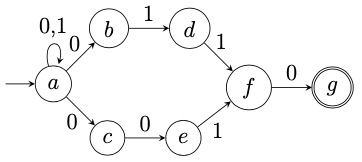
\includegraphics[width=0.7\columnwidth]{images/Screen Shot 2022-11-24 at 12.48.47.png}  
    \end{center}

\section{ Equivalences of Models}
\begin{center}
   \begin{tabular}{l c l l}
    RE & $\overset{\text{Th. 2.1}}{\longrightarrow}$ & $\epsilon-$NFA & $\mathcal{O}(|\alpha|)\\ \hline
    $\epsilon-$NFA & $\longrightarrow$ & NFA & $\epsilon-$closures $|Q|$\\ \hline
    $\epsilon-$NFA & $\overset{\text{Th. 3.2}}{\longrightarrow}$ & DFA & Powerset $2^{\mathcal{O}(|Q|)}$\\   \hline
    DFA & $\overset{\text{Th. 3.1}}{\longrightarrow}$ & NFA & Powerset $2^{\mathcal{O}(|Q|)}$\\ \hline
    DFA & $\longrightarrow$ & RE & State elim $4^{\mathcal{O}(|Q|)}$\\
    
    
\end{tabular} 
\end{center}


%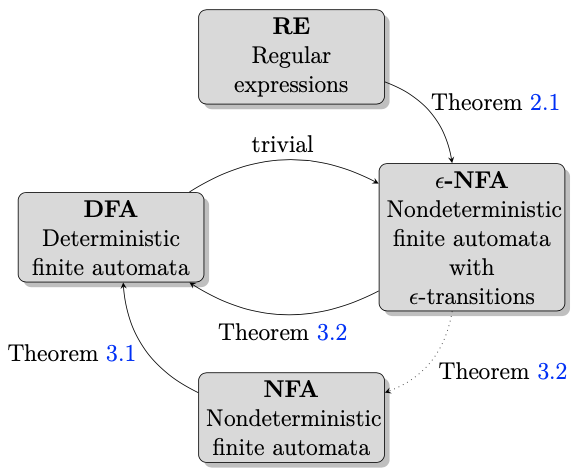
\includegraphics[width=\columnwidth]{Screen Shot 2022-12-24 at 12.15.28.png}

\subsection{From NFAs to DFAs}


\begin{theorem}
    For each NFA $\mathcal{A}$ exists a DFA $\mathcal{A}_D$ with $L(\mathcal{A}_D) = L(\mathcal{A})$
\end{theorem}

\subsubsection{Powerset Automaton}
After reading a word $w$, the state of $\mathcal{A}_D$ should be the set of all states $\mathcal{A}$ for which there exists a run from initial state reading $w$

Convert the follwoing NFA to a DFA  using the input $1011$ as a guide. 
\begin{center}
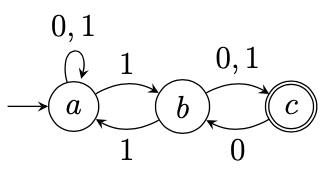
\includegraphics[width=0.5
\columnwidth]{images/Screen Shot 2022-12-24 at 13.00.46.png}
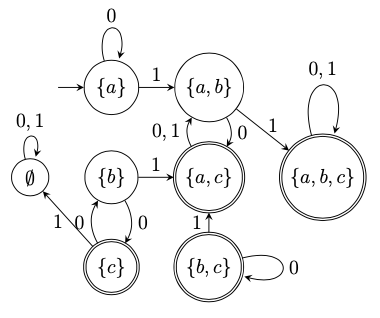
\includegraphics[width=0.8\columnwidth]{images/Screen Shot 2022-12-24 at 13.14.52.png}

\end{center}

Don't forget to put the empty state $\emptyset$. Or write that all missing transitions lead to a sink state

\subsection{From $\epsilon$-NFAs to DFAs}


\begin{theorem}
    For each $\epsilon$-NFA $\mathcal{A}$ exists a DFA $\mathcal{A}_D$ with $L(\mathcal{A}_D) = L(\mathcal{A})$
\end{theorem}

Very similar to the transformation of NFAs into DFAs with two differences:
\begin{itemize}
    \item Initial state: $\epsilon$-closure(s)
    \item $\delta_D(S, \sigma)= \epsilon-$closure$(\{q \, |\, \exists \, p \in S: p \overset{\sigma, \mathcal{A}}{\to} \})$
 \end{itemize}
 \begin{center}
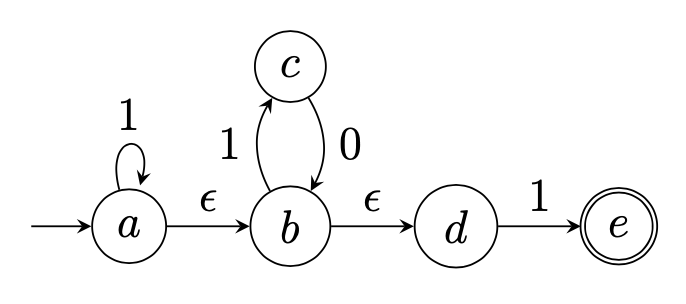
\includegraphics[width=0.7\columnwidth]{images/Screen Shot 2023-01-07 at 16.42.05.png}
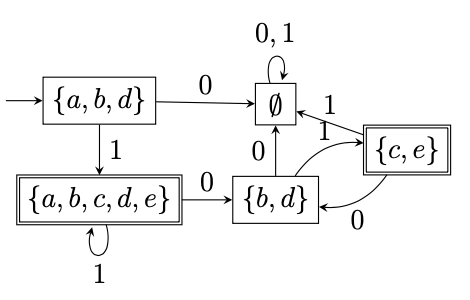
\includegraphics[width= 0.7\columnwidth]{images/Screen Shot 2023-01-11 at 12.09.29.png}
 \end{center}\textbf{$\epsilon$-closure}(p) Set of all reachable states from $p$ without reading a symbol) $\epsilon$-closure$(a) = \{a,b,d\}$
\subsection{From REs to DFAs}
\begin{tabular}{l l}
    $\sigma$ of an RE & \vcenter{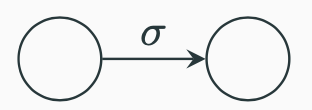
\includegraphics[width=1.4cm]{images/RE to DFA01.png}}  \\
     Concatenation & \vcenter{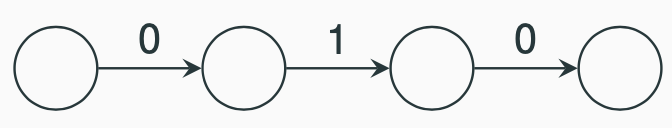
\includegraphics[width=3cm]{images/RE to DFA02.png}}\\
     \\ Repetition & \vcenter{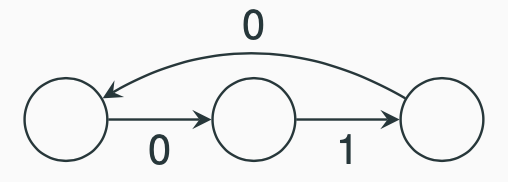
\includegraphics[width=2.3cm]{images/RE to DFA04.png}} \\
     Choice & \vcenter{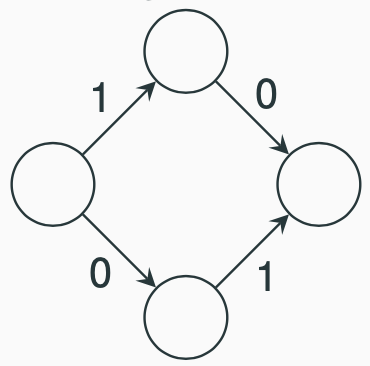
\includegraphics[width=1.8cm]{images/RE to DFA03.png}} 
\end{tabular}

\subsection{From DFAs to REs}

\begin{theorem}
    \textbf{McNaughton, Yamada} For each DFA $\mathcal{A}$ there exists an RE $\alpha$ with $L(\alpha) = L(\mathcal{A})$
\end{theorem}

\paragraph{State Elimination}
\begin{itemize}
    \item We use a hybrid automaton, whose transitions are labeled with regular expressions
    \item By successively removing states, a single regular expression is finally obtained
\end{itemize}

\begin{center}
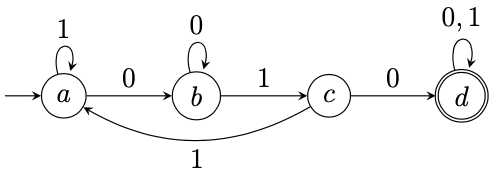
\includegraphics[width= 0.67\columnwidth]{images/Screen Shot 2023-01-07 at 16.37.09.png}
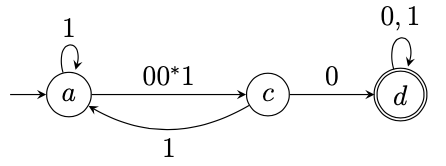
\includegraphics[width= 0.67\columnwidth]{images/Screen Shot 2023-01-07 at 16.37.19.png}
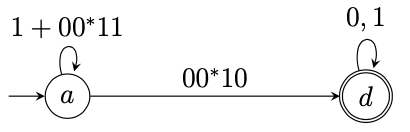
\includegraphics[width= 0.67\columnwidth]{images/Screen Shot 2023-01-07 at 16.37.32.png}
\end{center}

Giving us $(1 + 00^*11)^*00^*10(0 + 1)^*$

\subsection{Structural Induction}

%\begin{itemize}
%    \item The definition of regular expressions is an example for an \textbf{inductive definition} of a set:
 %   \item First, certain basic elements of the set are defined: $\emptyset, \epsilon, \sigma, \forall \sigma \in \Sigma$
 %   \item Then it is described how new elements can be constructed out of given elements of the set: Through concatenation, choice, repetition
 %   \item The set then consists of all elements which can be constructed in this way (in finitely many steps), and no other elements
 %   \item A well-known example of an inductive definition:
 %   \begin{itemize}
  %      \item $0 \in \mathbb{N}_0$
  %      \item $n \in \mathbb{N}_0 \implies n+1 \in \mathbb{N}_=$
  %  \end{itemize}
 %   \item Inductive definitions of sets allow for:
 %   \begin{itemize}
   %     \item Inductive definitions of functions on the elements of the set
   %     \item Inductive proofs of properties of all elements in the set, called \textbf{structural induction}
 %   \end{itemize}
%\end{itemize}

%\subsubsection{Inductive definitions of functions}
%\begin{itemize}
  %  \item We know that the set $\Sigma^*$ of all strings over $\Sigma$ can be defined inductively:
  %  \begin{itemize}
   %     \item $\sigma \in \Sigma^*$
   %     \item If $w \in \Sigma^*$ and $ \sigma \in \Sigma$, then $w \cdot \sigma \in \Sigma^*$
 %   \end{itemize}
%\end{itemize}


\begin{itemize}
    \item Proofs by structural induction prove that all elements of an inductively defined set have a certain property by
    \begin{itemize}
        \item first proving the statement for the basic elements,
        \item and then for the “composite” elements
    \end{itemize}
\end{itemize}


%\subsubsection{Proof Method: Simulation}


%\subsubsection{Correctness Proofs for DFAs}


\section{Automata Minimization} 

\subsection{Basic Idea}

\begin{enumerate}
    \item Unreachable states can be removed
    \item States whose transitions lead to the same states and that are either all accepting or all nonaccepting can be merged
    \item Sink states can be merged
    \item In general: states that have the same acceptance behaviour for all subsequent input sequences (including $\epsilon$) can be merged
\end{enumerate}

\subsection{Equivalence class Automaton}

\begin{itemize}
    \item The minimization of a DFA for a language L is based on a simple idea: Let $x,y$ be two strings with $xz \in L \iff yz \in L \forall z$
    \begin{itemize}
        \item So, the strings have the same behaviour with respect to L for all “extensions” $z$
        \item Notation for this relation between $x$ and $y: x \sim_L y$. $\sim_L$ is an \textbf{equivalence relation}
    \end{itemize}
    \item Therefore, by reading either x or y, the states we reach are not distinguishable by reading any word starting from these states. $\implies$  We can merge these states into a single state
    \item The equivalence classes of $\sim_L$ define the states of minimal DFA for $L$. This DFA is called the \textbf{equivalence class automaton}
\end{itemize}

\paragraph{Equivalence Relation}
A binary relation that is \textbf{reflexive, symmetric, transitive}

\paragraph{Equivalence Class} of an equivalence relation $\sim$ is a maximal set $K$ of elements such that $x \sim y \forall x,y \in K$

\subsection{Nerode Relation} 
\begin{definition}
    (Nerode Relation). Let $L \subseteq \Sigma^*$ be a language. The \textbf{Nerode relation} $\sim_L$ on $\Sigma^*$ is defined as: $x \sim_L y \Leftrightarrow \forall z \in \Sigma^*$ it holds that: $xz \in L \Leftrightarrow yz \in L$.
\end{definition}
Note that it might be that $z=\epsilon$. Example: $[\epsilon]=\{ w \in L \ | \ w$ does not contain the subword $aaa$ and does not end with $a$\}
\paragraph{Proposition} If the index $(\sim_L) = k$ is finite $\implies \exists$ a DFA for $L$ with $k$ states
The \textbf{equivalence class automaton} $\mathcal{A}_L = (Q,\Sigma, \delta, s, F)$ for $L$ is defined as follows:\begin{itemize}
    \item $Q$ is the set of equivalence classes of $\sim_L$
    \item $s = [\epsilon]$
    \item $F= \{[x] | x \in L\}$
    \item $\forall x \in \Sigma^*, \sigma \in \Sigma: \delta([x], \sigma) = [x \sigma]$
\end{itemize}


\subsection{Lower Bounds for DFAs} 
\subsection{Myhill-Nerode Theorem} 
To prove a language is (not) regular: By showing it has (in)finite equivalence classes or construct a DFA, NFA or RE that recognizes it. 
\begin{theorem}
    Nerode-Hill
    A language is regular iff $\sim_L$ has a finite number of equivalence classes
\end{theorem}

%\subsubsection{Further Applications}

\subsection{Minimal Automaton: Uniqueness}

\paragraph{Isomorphism}
$\mathcal{A}_1$ and $\mathcal{A}_1$ are caleld isomorphic if a bijection $\pi: Q_1\to Q_2$ exists where:
\begin{enumerate}
    \item $\pi(s_1)=s_2$
    \item $\forall q \in Q_1$ it holds that $q \in F_1 \iff \pi(q) \in F_2$
    \item $\forall q \in Q_1$ and $\sigma \in \Sigma$ it holds that: $\pi(\delta_1(q,\sigma))=\delta_2(\pi(q),\sigma)$
\end{enumerate}
\subsection{Algorithms: DFA Minimization}
\begin{itemize}
    \item[$\to$] $\mathcal{A}_L$ is constructed by merging states from $\mathcal{A}$
    \item Two states $p,q$ from $\mathcal{A}$ can be merged, if they are equivalent according to: $\forall z \in \Sigma^*: \delta^*(p,z) \in F \iff \delta^*(q,z) \in F$
    \item The basic idea behind our algorithm is to first calculate which states can not be merged
    \item Therefore, we consider an algorithm that calculates the set $N(\mathcal{A})$ of \textbf{non-equivalent states:} $N(\mathcal{A})=\{(p,q)\:|\:p,q\in Q, \exists z: (\delta^*(p,z) \in F \notiff \delta^*(q,z) \in F)\}$
    \item The calculation is done inductively: \begin{itemize}
        \item Begin by computing pairs which are inequivalent due to $z=\epsilon$
        \item Afterwards, compute pairs which are inequivalent due to transitions to other inequivalent pairs
    \end{itemize}
\end{itemize}
\subsubsection{Minimization Algorithm}
\begin{itemize}
    \item Input: $\mathcal{A}=(Q,\Sigma,\delta,s,F)$
    \item Output: minimal DFA $\mathcal{A}$ with $L(\mathcal{A'}(=L(\mathcal{A})$
    \begin{enumerate}
        \item Remove all states of $\mathcal{A}$ which are not reachable from $s$
        \item Compute the relation $N(\mathcal{A})$ using the table filling algorithm
        \item Merge iteratively all unmarked state pairs into one state
    \end{enumerate}
    \item Total runtime complexity: $\mathcal{O}(|Q|^2 \: |\Sigma|)$

\end{itemize}
\subsubsection{Table filling algorithm}
\begin{center}
    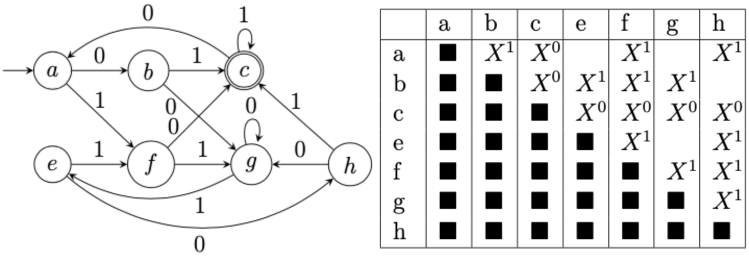
\includegraphics[width=\columnwidth]{images/Artboard.png}
\end{center}

\begin{itemize}
    \item Input: $\mathcal{A}=(Q,\Sigma,\delta,s,F)$
    \item Output: Relation $N(\mathcal{A})$ \begin{enumerate}
        \item $N = \{(p,q),(q,p)\:|\:p\in F,q\notin F$
        \item $N' = \{(p,q) \notin N \:|\: \exists \sigma \in \Sigma: (\delta(p,\sigma),\delta(q,\sigma))\in N)\}$ %e.g. states a and b. Using the symbol 1, a goes to f and b goes to c. But since the cell for (c,f) is already marked, we know that those states are not equivalent.
        \item $N = N \cup N'$
        \item If $N' \neq \emptyset$, continue with 2
        \item Output N
    \end{enumerate}
\end{itemize}



\subsubsection{Form an RE to a DFA: In Full}
\begin{enumerate}
    \item Specify the language by a regex $\alpha$
    \item Convert $\alpha$ into an $\epsilon-$NFA $\mathcal{A_1}$
    \item Convert $\mathcal{A_1}$ into a DFA $\mathcal{A_2}$
    \item Convert $\mathcal{A_2}$ into a minimal DFA $\mathcal{A_3}$
\end{enumerate}

\subsection{Further Insights}
\hl{The Myhill Nerode Theorem can be used to show a language is (not) regular} (Even though the pumping lemma is more suitable to show it is not). By demonstrating a language has (in)finitely many equivalence classses. To verify a set of equivalence classes one has to show: \begin{enumerate}
    \item Every string appears in a class
    \item $\forall u,v$ in the same class it holds that $u \sim_L v$
    \item[2']  All strings v of a class have the same set $L/v$
    \item For the strings $u, v$ from different classes it holds that $u \nsim_L v$
    \item[3'] Different classes have different sets $L/v$
\end{enumerate}

$L/v$ is the set of all strings than can be appended to $v$ such that the final word is in $L$.
\subsection{Minimal NFAs}
For every NFA A there is also a minimal NFA A′ with L(A′) = L(A). However, in general, minimal NFAs are not unique up to isomorphism!
\section{Limits, Closure Properties, Algorithms} 
\subsection{\hl{Pumping Lemma}}
\begin{itemize}
    \item Can show that a language is \textbf{not} regular
    \item Does not always work
    \item Can't be used to prove that a language is regular
    \item A 'cycle' in an accepting path can be repeated arbitrarily often
    \item If $\exists$ more words then equivalence classes ($|w| \geq |Q|) \implies \exists$ a state that the DFA visits (at least) twice while reading $w$\end{itemize} 
   
   \begin{theorem}
       (Pumping Lemma).
   $L$ is regular $\implies \exists \: n$ s.t. each $w \in L$ with $|w| \geq n$ can be decomposed into $xyz$ s.t. that:(1) $y \neq \epsilon$ \\(2) $|xy|\leq n$
        (3) $\forall k \geq 0: xy^kz \in L(\mathcal{A})$   \end{theorem}
Contraposition more useful

\begin{corollary}
    Let $L$ be a language. Assume that for each $n>0 \ \exists$ a string $w \in L$ with $|q|\geq n$ s.t. for each decomposition $w=xyz$ with (1) $y \neq \epsilon$ (2) $|xy|\leq n$ there $\exists$ a $k\gew 0$ s.t. $xy^kz \notin L \implies$ not regular. 
\end{corollary}

\paragraph{\hl{Example}}
$L_{a<b}$=\{w \in \{a,b\}^* | \#_a(w) < \#_b(w)\}$

Let $n \in \mathbb{N}$ be arbitrary. Choose $w=a^nb^{n+1}\in L_{a<b}:$ $\Rightarrow |w|=2n+1\geq n$

Let $x,y,z$ be arbitrary strings with $w=xyz$ and: (1) $y \neq \epsilon$ (2) $|xy|\leq n$. Due to (2), $y$ does not contain any $b$. Due to (1), $y$ contains at l. one $a$.

Choose $k \geq 2$:\\
$\Rightarrow xy^2z$ contains at least $n+1$ $a$'s but at most $n+1$ $b$'s\\
$\Rightarrow xy^2z \notin L_{a<b}$\\
$\Rightarrow L_{a<b}$ is not regular.

\begin{theorem}
    (Jaffe, 78). L is regular $\iff \exists \ n$ s.t. each string $w \in L$ with $|w|\geq n$ can be written as $w=xyz$ in at least one way s.t. condiitons hold: $(1) y \notin \epsilon (2) |xy| \leq n (3) \forall k\geq 0: xy^kz \sim_L xyz$ \
\end{theorem}

all $xyk^z$ have to be in the same Nerode equivalence class as $xyz$

\subsection{Regular Languages: Counting} We’ve encountered the intuitive criterion that a language is regular if it suffices to remember a constant amount of information while reading a word, independently of the input length.

\subsection{Closure Properties and Synthesis of Automata}
\subsection{Synthesis of Finite Automata}
%we are not concerned with the closure properties of individual languages, but with the closure properties of the class of all regular languages!
\subsubsection{Boolean Operations}
\begin{theorem}
    Let $\mathcal{A}_1, \mathcal{A}_2$ be DFAs.Then, DFAs can be constructed for the follwoing languages: 
    \begin{tabular}{l l l}
         &  States & Time \\
        $L(\mathcal{A}_1) \cap L(\mathcal{A}_2)$ & $|Q_1||Q_2|$ &  $\mathcal{O}(|Q_1||Q_2||\Sigma|)$\\
        $L(\mathcal{A}_1) \cup L(\mathcal{A}_2)$ & $|Q_1||Q_2|$ &  $\mathcal{O}(|Q_1||Q_2||\Sigma|)$\\
        $\Sigma^* - L(\mathcal{A}_1)$ & $|Q_1|$ & $\mathcal{O}(|Q_1|)$
    \end{tabular}
\end{theorem}

\begin{corollary}
    The class of reg. languages is closed for intersection, union and complementation.
\end{corollary}

%For the proof of intersection and union we will use a product automaton

\paragraph{\hl{Product automaton}}
\begin{center}
    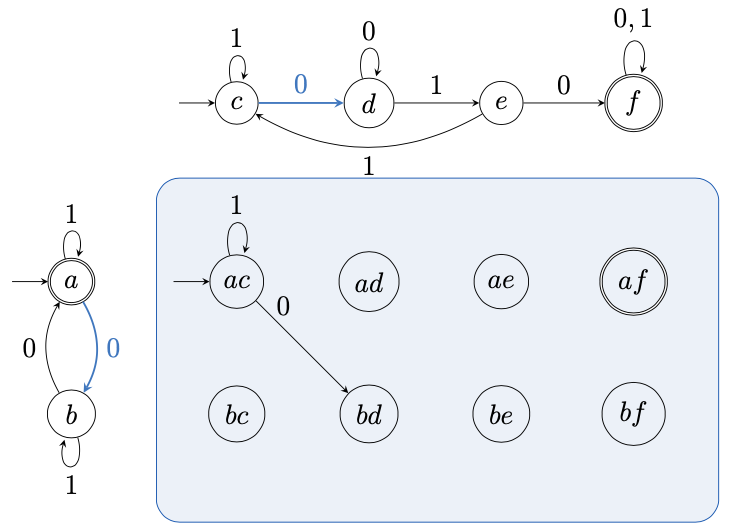
\includegraphics[width=0.9\columnwidth]{images/Screen Shot 2023-01-11 at 14.21.54.png}
\end{center} \begin{enumerate}
    \item Determine initial and accepting state. Only when both accept
    \item Add transitions
    \item Remove unreachable states!
\end{enumerate}


\subsubsection{Size}
\begin{center}
    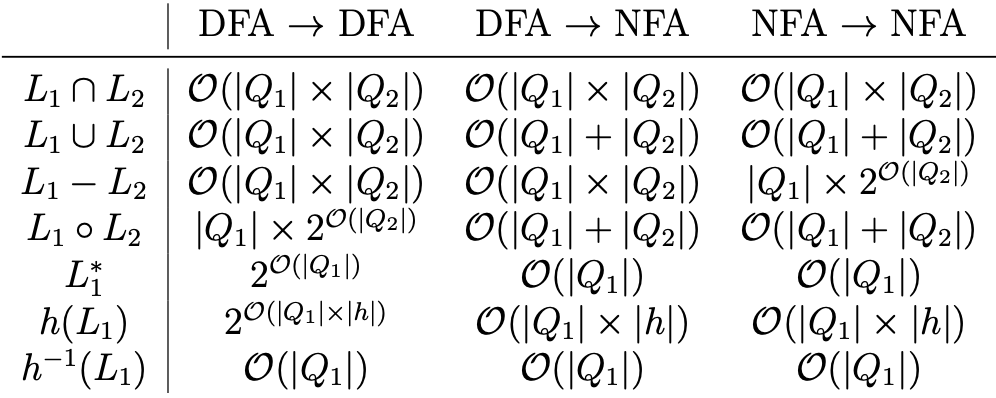
\includegraphics[width=0.97\columnwidth]{images/Screen Shot 2023-01-12 at 15.29.59.png}
\end{center}
\subsection{Closure Properties Reg Lang}

\subsubsection{Closure: Concatenation \& Iteration}

\stepcounter{theorem}
\stepcounter{theorem}

\begin{theorem}
    Let $\mathcal{A}_1,\mathcal{A}_2$ be DFAs (or NFAs) for $L_1, L_2$. Then DFAs (or NFAs) can be constructed for $L_1 \circ L_2$ and $L_1^*$
\end{theorem}
\subsubsection{Closure: Homomorphism}

\begin{definition}(Homomorphism)
A function $h: \Sigma^* \to \Gamma^*$ is a \textbf{homomorphism} if for all strings $u,v \in \Sigma^*: h(uv)=h(u)h(v)$.\end{definition} From the definition it follows that $h(\epsilon)=\epsilon$

\begin{theorem}
    If L over $Sigma$ and $\Gamma$ is an alphabet, then h(L) for each homomorphism h: $\Sigma^* \to \Gamma^*$
    is regular.
\end{theorem}
\subsection{Further Algos for Automata}
\subsubsection{Emptiness Test}
\begin{enumerate}
    \item Forget the edge labels
    \item Insert a target node $t$ and edges from all accepting nodes to t \item Test if there is a path from $s$ to $t$
    \item If yes: output “$L(\mathcal{A}) \neq \emptyset$”
\end{enumerate}

It might be simpler to backwards, from $t$ to $s$

\subsubsection{Word Problem}
Check if specific word in a given language

\begin{tabular}{l l l}
    DFA & simulate & $\mathcal{O}(|w|+\delta)$\\
    NFA & simulate powerset aut. & $\mathcal{O}(|w|\times \delta)$\\
    RE & $\to \epsilon$-NFA sim. powset aut. & $\mathcal{O}(|w| \times \alpha)$
\end{tabular}

\subsubsection{Equivalence Test for DFAs}
\hl{Two finite automata are equivalent if they decide the same language.} You can show that two automata are not equivalent by giving a word that is accepted by one of the automata but not by the other. To show that two automata are equivalent, use (1) or (2)
\paragraph{(1) With minimal Automata}
\begin{itemize}
    \item Construct min. automata $\mathcal{A}_1'$ and $\mathcal{A}_2'$
    \item Test if $\mathcal{A}_1'$ and $\mathcal{A}_2'$ are isomorphic \begin{itemize}
        \item Construct step-wise bijection $\pi$ from (the states of) $\mathcal{A}_1'$ to $\mathcal{A}_2'$
        \item Initialization: $\pi$ maps the initial state onto the initial state
        \item Then: Continue $\pi$ according to the transitions of $\mathcal{A}_1'$ and $\mathcal{A}_2'$
        \item "Both DFAs are now isomorphic according to $a \to c$ and $b \to d \Rightarrow$ DFAs are equiv." Also draw the graphs!
    \end{itemize}
\end{itemize}

\paragraph{(2) With product Automata}
\subsubsection{Equivalence Test for NFAs and REs}
The problem is (likely) even harder than NP.

\subsubsection{Finiteness Test}
We know that if we can pump a word, we can repeat a cycle over and over again, which would mean that the language is infinite. On the other hand, if there are no loops or cycles, the language must be finite.

\begin{theorem}
    The language of a DFA is infinite $\Rightleftarrow \exists$ state $q$ with:\begin{itemize}
        \item q is reachable from s,
        \item q lies on a cycle,
        \item An accepting state is reachable from q
    \end{itemize}
\end{theorem}
\section{Context-Free Language (1)} 

Prove a language is context-free: construct PDA.
 \paragraph{Context-free grammar (CFG)} $G=(V,\Sigma, S, P)$ consists of  \begin{itemize}
     \item finite set $V$ of \textbf{variables}
     \item an alphabet $\Sigma$
     \item a \textbf{start symbol} $S \in V$
     \item finite set $P$ of \textbf{rules}: $P \subseteq V \times (V \cup \Sigma)^*$
 \end{itemize}
 where $\Sigma \cap V = \emptyset$ has to hold
 
 \paragraph{Notation and terminology} \begin{itemize}
     \item Instead of $(A,BC) \in P$ we write $A \to BC$
 \begin{itemize}
         \item Elements of $V \cup \Sigma$: \textbf{symbols}
         \item Elements of $\Sigma$: \textbf{terminals}
         \item Elements of $V$: \textbf{nonterminals}
         \item Rules in $P$: \textbf{Productions}
     \end{itemize}
 \end{itemize}
 
 \subsection{Semantics}
 
 \paragraph{Derivation} 
 \begin{itemize}
     \item A derivation is a sequence of derivation steps
     \item In a derivation step a variable $X$ is replaced by the right-hand side $\gamma$ of a rule $X \to \gamma$ e.g: $bSB \Rightarrow_G baSab$
 \end{itemize}

\paragraph{Derivation Step}
\begin{itemize}
    \item Let $G=(V,\Sigma, S, P)$ be a context-free grammar
    \item A string of terminals and non-terminals of $G$ is a string from $(V\cup\Sigma)^*$
    \item If $u$ and $v$ are such strings of $G$, then $v$ results from $u$ in a \textbf{derivation step} if \begin{itemize}
        \item $u = \alpha X\beta$
        \item $v = \alpha \gamma \beta$
    \end{itemize}
    for \begin{itemize}
        \item a variable $X$
        \item $\mathtt{\alpha, \beta, \gamma \in (V \cup \Sigma)^*}$
        \item a rule $X \to \gamma$ in $P$
    \end{itemize}
    \item Notation: \textbf{$u\Rightarrow_G v$}
\end{itemize}

\subsection{Derivation Trees}
\begin{tabular}{l l}
     $A \to$ & $B \ | \ A+A \ | \ A \times A \ | \ (A)$\\ $B \to$ & $Ba \ | \ Bb \ | \ B0 \ | \ B1 \ | \ a \ | \ b$ 
\end{tabular}
    
\begin{center}
   \begin{tabular}{c c}
      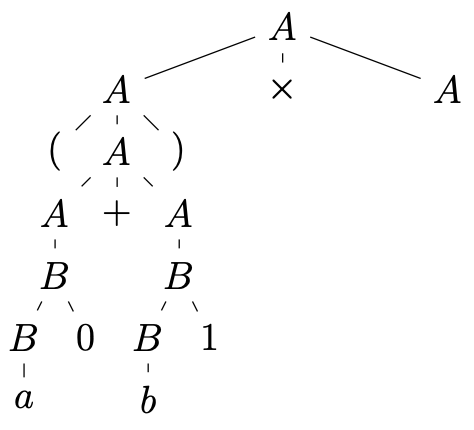
\includegraphics[width=0.5\columnwidth]{images/Screen Shot 2023-01-11 at 17.39.38.png}    &  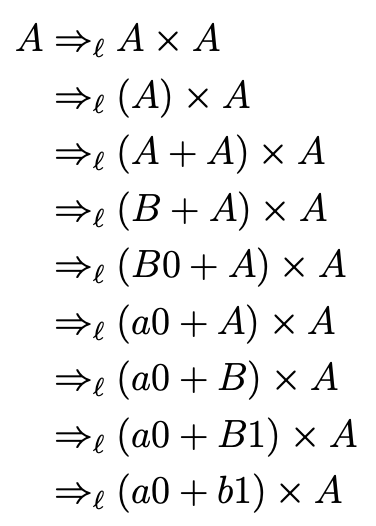
\includegraphics[width= 0.37\columnwidth]{images/Screen Shot 2023-01-11 at 17.39.41.png}
    \end{tabular}
\end{center}
This is a derivation tree for the string $(a0+b1)\times a+b$. \textit{!When asked for a derivation write down the derivation, not the derivation tree! Put the $l$}

\subsubsection{Leftmost Rightmost Derivations}
\begin{itemize}
    \item In each step, the left-/rightmost variable is replaced. 
    \item For each derivation tree, there exist corresponding leftmost and rightmost derivations. 
    \item Leftmost and rightmost derivations are not necessarily unique in a tree
    \item There are derivations that are neither leftmost nor rightmost
\end{itemize}



\subsection{Ambiguity}
For a given grammar and string  there are multiple derivations. Unfortunately, there is no general procedure to test if a grammar is unambiguous.

\paragraph{Ambiguous grammar} (Definition) A context-free grammar $G$ is called ambiguous if there exists a string $w$ which admits two different derivation trees with respect to $G$.
If there is only one derivation tree, G is called unambiguous.

\subsection{Extended CFGs}  allowing for more compact representations while preserving the semantics.

\paragraph{Extended Context-free grammar (CFG)} $G=(V,\Sigma, S, P)$ consists of  \begin{itemize}
     \item set $V$ of \textbf{variables}
     \item an alphabet $\Sigma$
     \item a \textbf{start symbol} $S \in V$
     \item finite set $P$ which contains exactly one  \textbf{rule}: $X \to \alpha_x$ for each variable $X \in V$ where $\alpha_x$ is a regular expression over $V \union \Sigma$
 \end{itemize}
 where $\Sigma \cap V = \emptyset$ has to hold

\section{Normal Forms} 

\subsection{Chomsky Normal Form (CNF)}
%Only allows rules of the form: %\begin{itemize}
 %   \item $X \to YZ$
  %  \item $X \to \sigma$
   % \item If necessary the rule $S \to \epsilon$ can be added
%\end{itemize} 

\subsubsection{Useful Symbol}
A symbol $X$ of a grammar is called useful if $X$ appears in a derivation $S \Rightarrow_G^* w$ of a word $w \in \Sigma^*$ In the grammar: $S \to AB | C$;
 $A \to b$;
 $C \to ab$;
$D \to c$. Only $S$ and $C$ are useful: they appear in the (only) derivation $S \Rightarrow C \Rightarrow ab$. $A, B,D$ are all not useful. $A$ is not useful because it can only be derived from $S$ along with $B$, which has no rule.

\begin{definition}
    Chomsky Normal Form, CNF\\
    $G = (V,\Sigma, S, P)$ is in \textbf{Chomsky normal form} if \begin{itemize}
        \item $G$ only contains useful symbols
        \item All rules of $G$ are of the form \begin{itemize}
            \item $X \to YZ$
            \item $X \to \sigma$
        \end{itemize} with $X,Y,Z \in \Sigma$
        \item If $S$ does not appear on the right-hand side of any rule, the rule $S \to \epsilon$ is allowed
    \end{itemize}
\end{definition}

\begin{theorem} (Chomsky 59)
\begin{itemize}
    \item For every context-free language $L$, there exists a grammar $G$ in CNF with $L(G)$ = $L$. 
    \item Any given grammar $G_0$ for $L$ can be brought in CNF in time $\mathcal{O}(|G_0|^4)$.
\end{itemize}
\end{theorem}

\subsection{\hl{Conversion to CNF}} 

\begin{enumerate}
    \item[$(G_1)$] Only useful symbols are allowed.
    \begin{enumerate}
        \item Remove non-generating rules
        \item Remove non reachable rules     \end{enumerate}
    \item[$(G_2)$] Right-hand sides contain exactly one terminal symbol or only variables: \begin{enumerate}
        \item For every terminal symbol $\sigma$: Insert a new variable $W_\sigma$ and replace $\sigma$ by $W_\sigma$ everywhere on the right-hand side, incl. in rules but only replace symbols $\sigma$ not variables $X$!
        \item Insert a new rule $W_\sigma \to \sigma$
    \end{enumerate}
    \item[$(G_3)$] No $X \to \beta$ rules with $|\beta| > 2$ are allowed: \\ We only have to look at the rules containing more than two variables. The first would be $S \to W_bDD$. To shorten this, we introduce a new proxy-variable $S_1$ and add the rules $S \to W_bS_1$ and $S_1 \to DD$.
    \item[$(G_4)$] No $\epsilon$-rules allowed\begin{enumerate}
        \item compute the set $V_{\epsilon}$ of all variables $Y$ with $Y\to^* \epsilon$
        \item $\forall$ right-hand side occurrence $X \to YZ$ or $X \to ZY$ of these variables, add new rules $X \to Z$
        \item eliminate all rules of the form $X \to \epsilon$
        \item remove useless variables (1) non-generating (2) non-reachable
    \end{enumerate} 
    \item[$(G_5)$] No unit rules ($X \to Y$) allowed:
    compute all pairs $U = \{(XY) \ | \ X \Rightarrow^* Y, X \neq Y \}$ . For these pairs, check if a non-unitrule $Y \to \alpha$ occurs, and if so, a new rule $X \to \alpha$ is added. $Y \to \alpha$ is a non-unit rule if $α = Z_1Z_2$ or $\alpha = \sigma$ (two variables or a terminal symbol).\\ Eliminate unit rules\\
    \item[$(G_6)$] If language L contains the string $\epsilon$: 
if $S$ does not appear on the right-hand side of any rule then Insert the rule $S \to \epsilon$. Else: Insert a new start symbol $S′$ and the rule $S′ \to \epsilon$

\end{enumerate}
%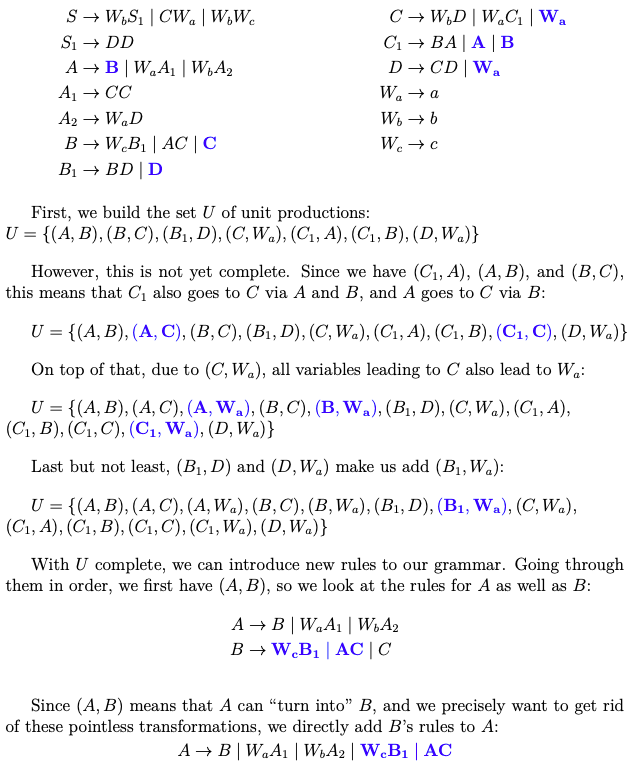
\includegraphics[width=\columnwidth]{images/Screen Shot 2023-01-11 at 21.36.41.png}

\section{Pushdown Automata} 

\subsection{Definition}
A pushdwon automaton (PDA) $\mathcal{A}=(Q,\Sigma,\Gamma, \delta, q_0, \tau_0, F)$ consists of \begin{itemize}
    \item finite set of states $Q$
    \item input alphabet $\Sigma$
    \item stack alphabet $\Gamma$
    \item finite transition relation $\delta \subseteq (Q \times (\Sigma \cup \{\epsilon\}) \times \Gamma) \times (Q \times \Gamma^*)$
    \item initial state $q_0 \in Q$
    \item initial stack symbol $\tau_0 \in \Gamma$
    \item set $F$ of accepting states
\end{itemize}

\begin{center}
    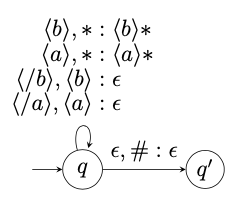
\includegraphics[width=0.45\columnwidth]{images/Screen Shot 2022-12-26 at 15.58.02.png}
\end{center}

The only visible difference to finite automata lies in the transitions. 
\subsubsection{Transition relation $\delta$} ($p, \sigma, \tau, q, z$) \begin{itemize}
    \item $p$ current state
    \item $\sigma$ input symbol with $\sigma \in \{\Sigma \cup \epsilon\}$
    \item $\tau$ symbol on top of stack
    \item $q$ new state
    \item $z$ replace $\tau$ with $z$
\end{itemize}

Given a state ($Q$), an input symbol ($\Sigma \cup \{\epsilon\}$) and a symbol on the top of our stack ($\Gamma$), this leads us to another state ($Q$), and we might make changes on our stack ($\Gamma^*$).

Instructions of the form:
$$\langle b \rangle, *: \langle b \rangle*$$
\begin{center}
    input, top of stack : new top of stack
\end{center}

* not a stack symbol, can be substituted with any other symbol in the stack alphabet.

\subsubsection{Configurations}
Describe the current “situation”.

\begin{definition} (Configuration of a PDA)\\
Let A $\mathcal{A}=(Q,\Sigma,\Gamma, \delta, q_0, \tau_0, F)$ be a PDA. A \textbf{configuration} ($q, u, v$ of $\mathcal{A}$ consists of: \begin{itemize}
    \item a state $q \in Q$
    \item the remaining input $u \in \Simga^*$
    \item the stack content $v \in \Gamma^*$
\end{itemize}
Start configuration with input w: (s,w,\tau_0)
\end{definition}

\subsubsection{Configurations and Runs}

\begin{definition} (Sucessor Configuration) Let  $\mathcal{A}=(Q,\Sigma,\Gamma, \delta, q_0, \tau_0, F)$ be a PDA. The succesor configuration $\vdash_\mathcal{A}$ is defined as follows: \begin{itemize}
    \item $\forall p,q \in Q, \sigma \in \Sigma, \tau \in \Gamma, u \in \Sigma^*, z, v \in \Gamma^*$:
    \item $(p, \sigma u, \tau v) \vdash_\mathcal{A}(q, u, zv)$ if $(p, \sigma, \tau, q, z) \in \delta$
    \item $(p, u, \tau v= \vdash_\mathcal{A} (q, u, zv)$ if $(p, \epsilon, \tau, q, z) \in \delta$
\end{itemize}
If $; \vdash_\mathcal{A} K'$ then $K'$ is called a \textbf{successor configuration} of K
\end{definition}

\begin{definition}
    (Run of PDA). A run of a PDA $\mathcal{A}$ is sequence $K_1, \dots, K_n$ of configurations with $K_I \vdash_\mathcal{A} K_{i+1} \forall i \in \{1, \dots, n-1\}$
\end{definition}

\subsubsection{Accepting}

\subsection{Empty Stack vs. Accepting States}

\begin{theorem}
    For each PDA $\mathcal{A}$ whihc accepts with an empty stack, $\exists$ a PDA $\mathcal{B}$ which accepts with accepting states such thath $L(\mathcal{B})=L(\mathcal{A})$ and vice versa.
    
\end{theorem}
\subsubsection{Empty Stack $\to$ Accepting States}

\subsubsection{Accepting States $\to$ Empty Stack}

\subsection{CFGs $\equiv$ PDAs}
\begin{theorem}
For each context-free grammar G, there exists a pushdown automata $\mathcal{A}$ with $L(\mathcal{A}) = L(G)$
\end{theorem}
\centering
\begin{tabular}{c c}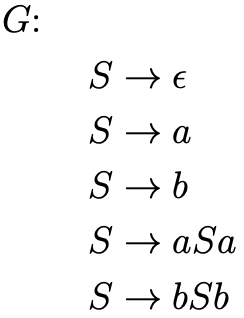
\includegraphics[align=t, width=0.26\columnwidth]{images/Screen Shot 2023-01-12 at 10.33.28.png} & 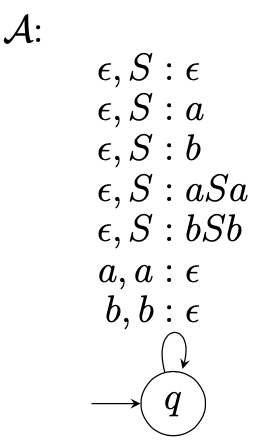
\includegraphics[align=t, width=0.28\columnwidth]{images/Screen Shot 2023-01-12 at 10.33.40.png} \\
\end{tabular}
\raggedright
%\begin{itemize}
    %\item Let $G=(V,\Sigma,S,P)$
    %\item The PDA $\mathcal{A}$ with input $w$ creates a leftmost derivation for a word $v$ and tests that $w=v$ holds
    %\item If the current sentential form begins with a terminal symbol, this symbol is subsequently compared with the next symbol of $w$.
%\item If there is a sentential form $uX\alpha$, a step in a leftmost derivation replaces the variable $X$ with a string $\beta$ according to a rule $X \to \beta$.
%\item In $\mathcal{A}$ this corresponds to $u$ already having been read and $X\alpha$ being the stack content.
%\item To implement the derivation step, A proceeds as follows:
%\begin{enumerate}
    %\item “Guess” the rule $X \to \beta$
    %\item Replace $X$ on the stack with $\beta$
   % \item Compare the leading terminal symbols of $\beta \alpha$  with the next symbols of the input and reduce them (i.e. delete them from the stack).
%\end{enumerate} 
%\end{itemize}


% MORE TO FILL IN!

\begin{theorem}
For each pushdown automaton $\mathcal{A} \ \exists$ a context-free grammar G with $L(G)=L(A)$ 
\end{theorem}

On a high level, we suppose that we have a PDA with initial stack symbol $\tau_0$ and that we are in the initial state $s$, and we want to read the input word $w$:
%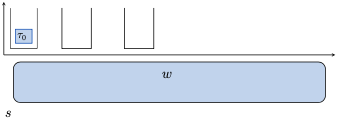
\includegraphics[width=\columnwidth]{images/Screen Shot 2022-11-10 at 16.55.59.png}

First step $\mathcal{A}$ replaces the initial stack symbol with a string $Z_1 \dots Z_k$ and reads a prefix $u_0$ of the input $w$:

%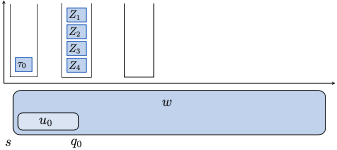
\includegraphics[width=\columnwidth]{images/Screen Shot 2022-11-10 at 16.57.41.png}

The symbols $Z_1 \dots Z_k$ are then successively deleted from the stack in the rest of the computation:

%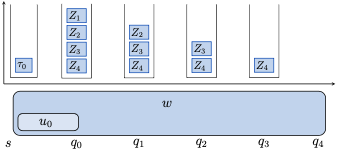
\includegraphics[width=\columnwidth]{images/Screen Shot 2022-11-10 at 16.59.16.png}

Thereby the substrings $u_1,\dots ,u_k$ of the input are read:

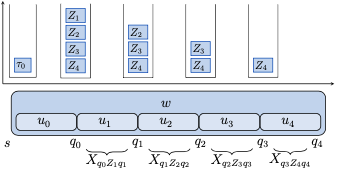
\includegraphics[width=\columnwidth]{images/Screen Shot 2022-11-10 at 17.00.38.png}

\paragraph{Idea for the grammar} For each combination $p,p' \in Q, \tau \in \Gamma$ the grammar $G$ contains a variable $X_{p,\tau , p'}$ which generates all strings for which $\mathcal{A}$ has a partial computation from state $p$ to state $p'$ which overall deletes the symbol $\tau$ from the stack.

\subsection{Deterministic PDAs}

%\subsubsection{Definition}
 In deterministic pushdown automata (DPDAs), there may only be one transition $(p, \sigma, \tau, q, w)$ in $\delta$ for each combination of $p,\sigma, \tau$.

We can have an $\epsilon$-transition going out of $q$ for stack symbol $\tau$, only if for the same state $q$ and stack symbol $\tau$, there is no further transition.  

$\exists \ (p, \epsilon, \tau, q ,w) \implies$ there may not be a transition $(p, \sigma, \tau, q', w')$ for any $\sigma$. 

\\(1) $(p, \epsilon, \tau, q_1, w_1)$
    (2) $(p, \epsilon, \tau, q_2, w_2)$


\section{Context-Free Language (2)} 

\subsection{\hl{Pumping Lemma}} To determine that a language is not context-free.

\subsection{Application}

\begin{corollary}
Let $L$ be a language. Assume that for each $n > 0 \exists$ a string $z \in L$ with $|z| \geq n$ such that for each decomposition $z=uvwxy$ with (1) $vx \neq \epsilon$ (2) $|vwx|\leq n$
$\exists$ a $k \geq 0$ where $uv^kwx^ky \notin L$ $\implies$ $L$ is not context-free.
\end{corollary}
 Let $n>0$ be arbitrary. Choose $z=a^nb^nc^n \in L, |z|\geq n$ holds. Let $uvwxy$ be a decomposition of $z$ with $u,v,w,x,y \in \{a,b\}^*$ satisfying (1) and (2). Due to $|vwx|\leq n$ and because there are $n$ $b$'s $vx$ can never consist of more than two different symbols. Choose $k=0: uv^0wx^0y=uwy \notin L$ since... $\Rightarrow L$ is not context-free
\begin{itemize}
    %\item $n$: cannot be chosen, the argument must work for arbitrary $n$
    %\item $z$ can be chosen freely from $L$ dependent on $n$, with $|z| \geq n$
    \item Decomposition $z$ in $uvwxy$ no choice can be made, the argument must work for arbitrary decompositions which fulfill $(1)$ and $(2)$
    \item $k$ can be chosen freely and individually for each possible decomposition $z$
    \item In the context-free pumping lemma $vwx$ can be anywhere in $z.$
\end{itemize}

\subsection{CFG Closure Properties}
%\subsubsection{Main Closure Properties}
\begin{theorem}
The class of context-free languages is closed under:  union, concatenation, the *–operator, the +–operator
\end{theorem}

%\subsubsection{Further Closure Properties}

\begin{enumerate}
    \item If $L$ is context-free then $\{w^R\: | \: w \in L \}$ is as well
    \item If $L \subseteq \Sigma^*$ is context-free and $h: \Sigma^* \to \Gamma^*$ a homomorphism, then $h(L)$ is context-free
    \item If $L \subseteq \Sigma^*$ is context-free and $h: \Sigma^* \to \Gamma^*$ a homomorphism, then $h^{-1}(L)$ is context-free 
\end{enumerate}

%\subsubsection{Missing Closure Properties}
\begin{theorem}
The class of context-free languages is \textbf{not} closed under: intersection, complementation, set difference.
\end{theorem}

\begin{theorem}
If $L_1$ is context-free and $L_2$ is regular, then $L_1 \cap L_2$ is context-free.
\end{theorem}

\subsection{Closure Propert of det.  CFGs}

\subsubsection{Closure Under Complementation}

\begin{theorem}
Deterministic context-free languages are closed under complementation.
\end{theorem}


\subsubsection{Union and Intersection}
The class of deterministic context-free languages is \textbf{not} closed under
union and intersection.

\subsubsection{Not all contxt-free-langs have a DPDA}
The class of deterministic context-free languages forms a proper subset of the class of context-free languages.

\subsection{Relation Between Classes}
\begin{theorem}
\begin{enumerate}
    \item Each regular language is deterministic context-free
    \item There are deterministic context-free languages which are not regular
    \item There are context-free languages which are not deterministic context-free 
\end{enumerate}
\end{theorem}
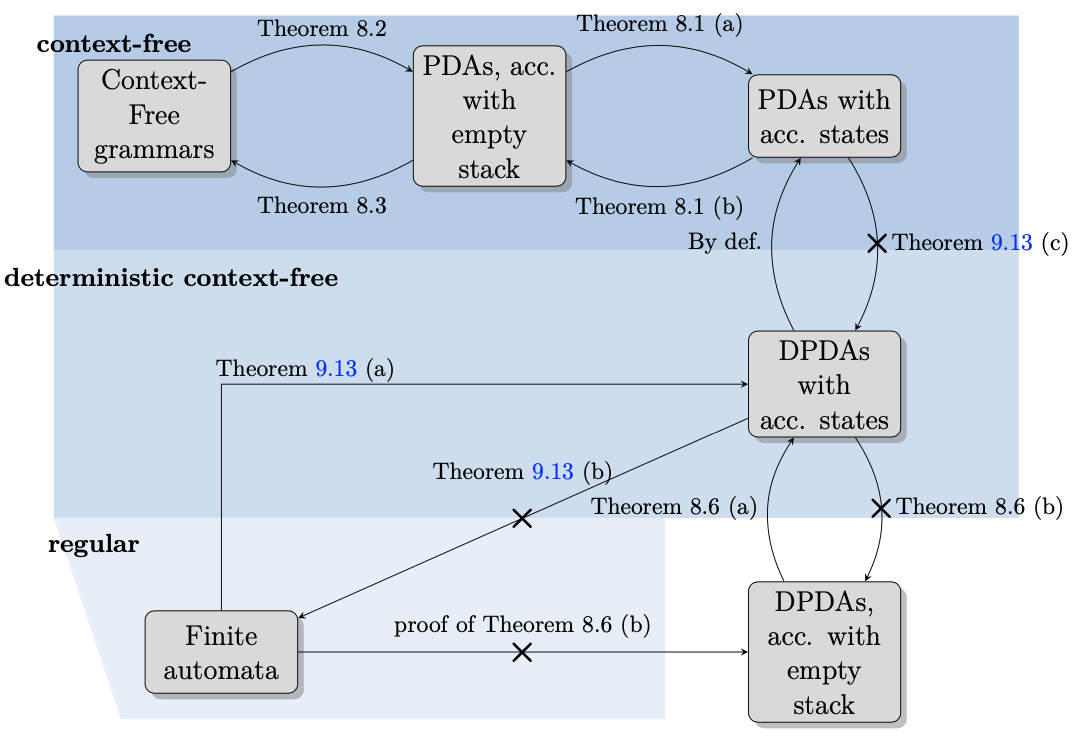
\includegraphics[width=\columnwidth]{images/Screen Shot 2022-11-11 at 14.26.35.png}

\section{Syntax Analysis}
Syntax analysis is used to verify whether a given program is syntactically correct
\subsubsection{Word Problem}

 

\begin{definition}
    (Word Problem for CFGs)
    Input: A word $w \in \Sigma^*$ and a grammar G.
    Output: Is $w \in L(G)$
\end{definition}

\begin{definition}
     (Syntax Analysis Problem for CFGs).
     Input: A word $w \in \Sigma^*$ and a grammar G.
     Desired output: If $w \in L(G)$: Derivation tree
\end{definition}

\subsection{Backtracking}

\subsubsection{Top-down Syntax Analysis}
The backtracking algo is “brute-force” iteratively trying all derivations $ S \Rightarrow_l^* w[1,m] X \alpha$ of the form $X\to \beta$ to generate the leftmost derivation. It's $\mathcal{O}(p^n)$ exp.

\subsection{CYK Algorithm}
\begin{itemize}
    \item Takes cubic time $\mathcal{O}(|w|^3|G|)$
    \item Uses dynamic programming
\end{itemize}

\paragraph{Solving the word problem}
\begin{enumerate}
    \item Write down the input word: $01110100$.
    \item Construct a triangular table. First row: one cell for each symbol of the input word, and each consecutive row has one symbol less: %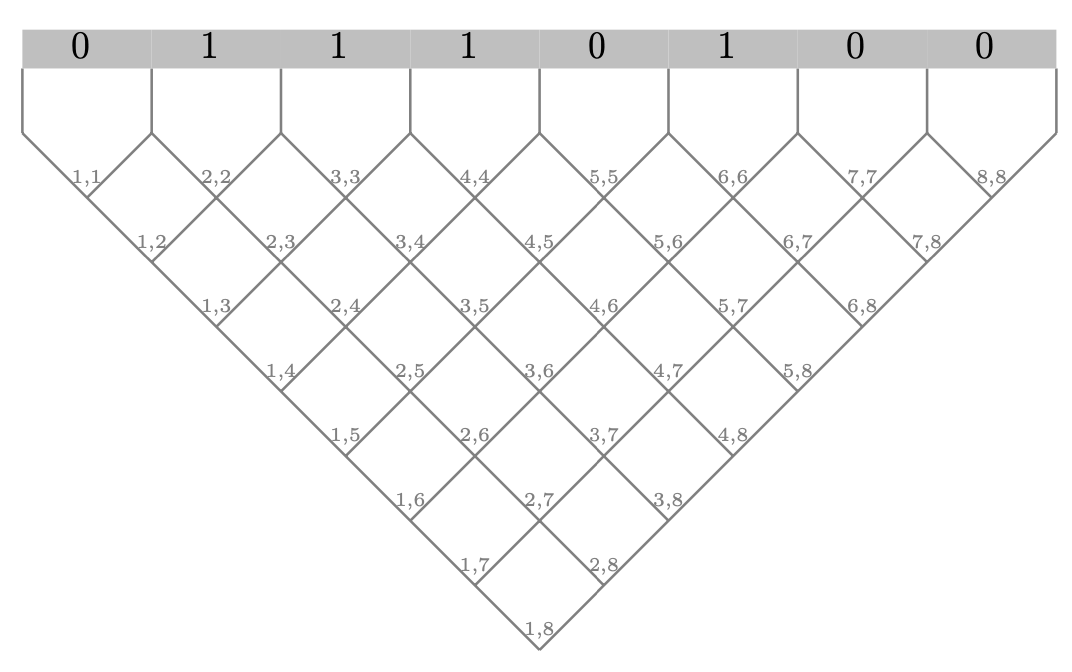
\includegraphics[width = \columnwidth]{images/Screen Shot 2022-11-21 at 15.22.05.png}
    The numbers at the bottom of each cell represent the indices. For example, the (4,6) cell represents the substring from 4 to 6.
    \item Fill the table. The first row check whether there is a rule that derives a given symbol.
    \item Next row. In cell (1,2) check for a rule that concatenates its children, (1,1) and (2,2).
    \item Cell (1,3), we cross over the results from the previous row. Concretely, we match (1,2) with (3,3) and (1,1) with (2,3).
    \item Continue until final cell,
    \item At this stage, we are particularly interested in S. Other variables would not be good enough.
\end{enumerate}

\subsubsection{Extended CYK ALgorithm}
For solving the \textit{syntax analysis problem} to obtain the derivation tree we extend the CYK algorithm slightly, to keep track of how we partitioned the word.
$B^2$ means we split between the second and third symbol
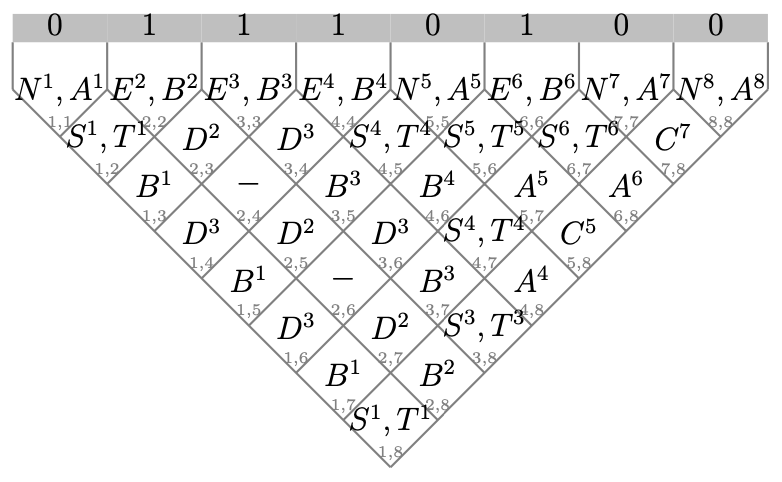
\includegraphics[width = \columnwidth]{images/Screen Shot 2022-11-21 at 16.10.19.png}
%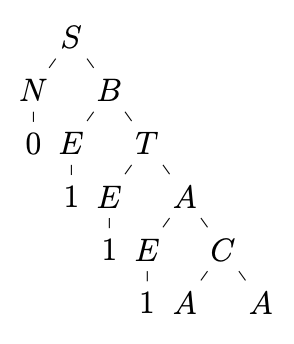
\includegraphics[width = 0.4 \columnwidth]{images/Screen Shot 2022-11-21 at 16.11.35.png}

\subsection{Top-Down Syntax Analysis}
Restricted CFG so syntax analysis can run in linear time and the next applicable rule only depends on the next input symbol.
%\subsubsection{Principles}
\stepcounter{subsubsection}

\subsubsection{LL(1) Grammars}


\begin{definition}
     (LL(1) Grammar). Let $G$ be a CFG without useless variables \& left-recursion. $G \in$ LL(1) if $\forall$ variables $X$ and rule $X \to \alpha, X \to \beta,$ with $\alpha \neq \beta$ the following conditions hold:
     \begin{enumerate}
         \item $FIRST(\alpha) \cap FIRST(\beta) = \emptyset$
         \item \hl{If $\alpha \Rightarrow^* \epsilon,$} then FOLLOW(X) $\cap$ FIRST($\beta)= \emptyset$
     \end{enumerate}

\end{definition}

For a sentential form $\alpha$, let \underline{\hl{FIRST($\alpha$)}}= \\ $\{ \sigma \in \Sigma \, | \, \alpha \Rightarrow^* \sigma v, v \in \Sigma ^* \} \cup \{ \epsilon \: | \: a \Rightarrow^* \epsilon \} $ {FIRST}($\alpha$) contains all first terminal symbols of strings that can be derived from $\alpha$, and possibly also $\epsilon$, if it can be derived from \alpha.

For a variable $X$ let \underline{\hl{FOLLOW(X)}}$=\{ \sigma \in \Sigma \, | \, S \Rightarrow^* uX\sigma v, u, v \in \Sigma ^* \}$ FOLLOW(X) contains all terminal symbols that may appear directly after $X$ in a sentential form for $X$.
\subsubsection{Look up table}
\begin{center}
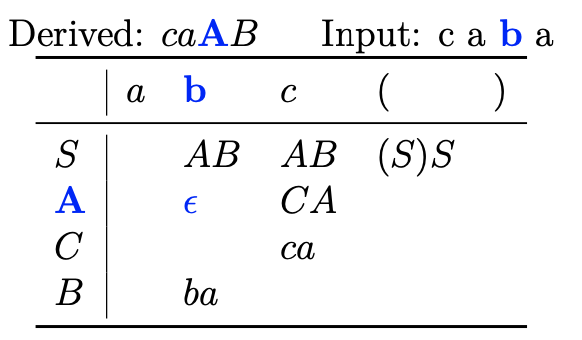
\includegraphics[width=0.6\columnwidth]{images/Screen Shot 2023-01-12 at 13.51.21.png}
\end{center}
Simply fill in the rules corresponding to terminal symbols and variables
%\subsubsection{Optimized Syntax Analysis}

%\subsubsection{Efficient Top-Down Syntax Analysis: Preliminary Considerations}

\section{Turing Machines}

\subsection*{Post Correspondence Problem} 

\subsubsection{Pseudo PCP}
\begin{center}
  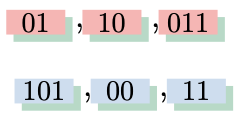
\includegraphics[width = 0.3\columnwidth]{images/Screen Shot 2022-11-23 at 11.26.39.png}
\end{center}

\begin{itemize}
    \item Given red \& blue blocks with strings
    \item An arbitrary number of blocks is available for each block type
    \item Is there a word that can be constructed from red blocks as well as from blue blocks?
\end{itemize}

\subsubsection{PCP}
\begin{itemize}
    \item Given a set of block types 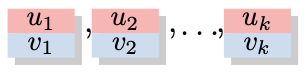
\includegraphics[width = 0.4\columnwidth]{images/Screen Shot 2022-11-23 at 11.51.41.png} 
    \item An arbitrary number of blocks is available for each block type.
    \item  Can the blocks be arranged in a line such that the red (upper) word equals the blue (lower) word?
\end{itemize}
\begin{definition}
     (PCP).\\
    \textbf{Input:} Sequence $(u_1,v_1), \dots , (u_k,v_k)$ of pairs of non-empty strings.\\
    \textbf{Question:} Is there an index sequence $i_1, \dots, i_n$ with $n \geq 1$ such that $u_{i_1} u_{i_2} \dots u_{i_n} = v_{i_1} v_{i_2} \dots v_{i_n}$?
\end{definition}

We call an index string $\Vec{i}=i_1, \dots, i_n$ a \textbf{solution} and the string $u_{i_1}u_{i_2}\dots u_{i_n}$ a \textbf{solution string}.

\begin{theorem}
PCP is not decidable.
\end{theorem}

\subsection{Turing Machines}
\subsubsection{Definition}
\begin{definition}
    (Turing Machine (Syntax))\\ $M=(Q,\Gamma, \delta, s)$ consists of:
    \begin{itemize}
        \item a finite set of states $Q$
        \item working alphabet $\Gamma$ with $\textvisiblespace, \rhd \in \Gamma$
        \item transition function $\delta$: \\ $Q \times \Gamma \to (Q \cup \{\text{yes, no}\}) \times \Gamma \times \{\leftarrow, \downarrow, \rightarrow\}$
        \item start state $s \in Q$
\end{itemize}
where it holds that $Q, \Gamma, \{\text{yes, no}\}$ and $\{ \leftarrow, \downarrow, \rightarrow\}$ are pairwise disjoint.
\end{definition}

\begin{itemize}
    \item  The symbol $\rhd$ signifying the left end of the tape must not be overwritten
    \item The head is not allowed to move left from $\rhd$
\end{itemize}

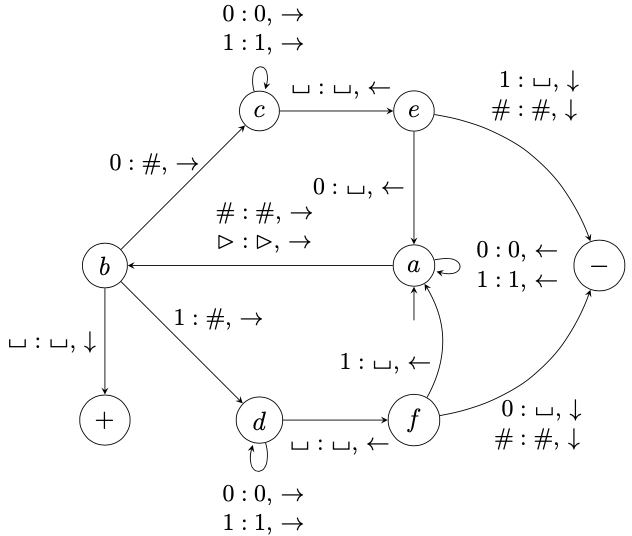
\includegraphics[width=\columnwidth]{images/Screen Shot 2022-12-26 at 17.14.00.png}
\subsubsection{Transitions}
\begin{center}
    \textit{before: after, move}
\end{center}
\begin{itemize}
    \item[$a$:] Read over 0 and 1; move left– if $\rhd$ or \# then move right; switch to $b$
    \item[$b$:] If 0 then overwrite it by \# and move right; switch to $c$...
\end{itemize}
\subsubsection{Configurations}
\begin{definition}
     (String-Tape Head Decription)
     (w,z) consists of \begin{itemize}
        \item a string $w \in \Gamma^*$
        \item a tape head position $z \ \mathbb{N}, 1 \leq z \leq |w|$
     \end{itemize}
\end{definition}

Sometimes the notation $(u, \sigma, v)$ is used instead of  $(w,z)$ with $w=u\sigma v$, and $|u \sigma|=z$. $(\rhd 10, 0, 00 \textvisiblespace)$

%That is, $w$ is divided into three substrings $u\sigma v$ where the length of $u \sigma$ equals the position of the tape head. For the example above: $(\rhd 10, 0, 00 \textvisiblespace)$
\begin{definition}
     (Configuration) of M is a tuple (q,(w,z)) consisting of \begin{itemize}
         \item a state $q \in Q \cup \{yes, no\}$
         \item a string-tape head description (w,z)
     \end{itemize}
\end{definition}

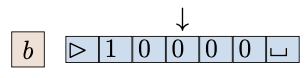
\includegraphics[width=0.45\columnwidth]{images/Screen Shot 2022-12-26 at 17.26.16.png} is $(b,(\rhd 10000 \textvisiblespace ,4))$
\begin{definition}
     (Successor configuration $\vdash_M$)\\ Let $K=(q,(w,z))$ be a configuration with $w[z]=\sigma$ and let $\delta(q,\sigma)=(q',\tau, d)$ with $\tau \in \Gamma, d \in \{\leftarrow, \downarrow, \rightarrow\}$.

     Then $K'=(q',(w',z'))$ is the successor configuration of K: $K \vdash_M K'$. We write $K \vdash_M^* K'$ if $\exists$ configurations $K_1, \dots, K_l$ with $K \vdash_M K_1 \vdash_M \dots \vdash_M K_l \vdash_M K'$
\end{definition}
\subsubsection{Semantics} When does a TM accept or reject? What does it's output for a particular input word mean?
\begin{definition}
    (TM (Semantics)) Let M be a TM. \begin{itemize}
        \item $\Sigma \subseteq \Gamma - \{\rhd, \textvisiblespace \}$ is called the \textbf{input/output alphabet}
        \item \textbf{Start configuration} with input $u \in \Sigma^*$ is $K_0(u)=(s,(\rhd u, 1))$
        \item $(q,(w,z))$ is called a \textbf{halting configuration} if $q \in$ \{yes, no\}
        \item $K_0, K_1, \dots, K_t$ is called a \textbf{finite computation of $M$ with input $u$} if: \begin{itemize}
            \item $K_0=K_0(u)$
            \item $K_i \vdash_M K_{i+1} \forall i<t$
            \item $K_t$ is a halting configuration
        \end{itemize}
        \item ...
    \end{itemize}
\end{definition}

If a TM is used to answer yes-no questions it can be described as follows:

\begin{definition}
    (Language decided by M). A TM M decides a language L if for each $u \in Sigma^*$: \begin{itemize}
        \item $u \in L \implies$ M accepts u
        \item $u \notin L \implies$ M rejects u 
    \end{itemize}
\end{definition}
TM has to halt for every possible input word.

\begin{definition}
    (L(M)) L(M)= set of all words accepted by M
\end{definition}
\subsubsection{Functions}
\begin{definition}
    $f_M(u)=v \in \Sigma^*$ if \begin{itemize}
        \item $K_0(u) \vdash_M^* (yes,(\rhd v,1))$ or
        \item $K_0(u) \vdash_M^* (yes,(\rhd v \tau w,1))$  for a $\tau \in \Gamma - \Sigma, w \in \Gamma^*$
    \end{itemize}
    $f_M(u)$ is undefined $(f_M(u)= \bot)$ if $\nexists$  such a v.
\end{definition}
Function-calculating TMs must finish with the head pointing on the starting symbol $\rhd$

\begin{definition}
    (Turing computable) A partial function $F: \Sigma^* \to \Sigma^* 
    $ is Turing computable if $f=f_M$ for a Turing Machine M
\end{definition}

\subsection{Multitape Turing Machines}
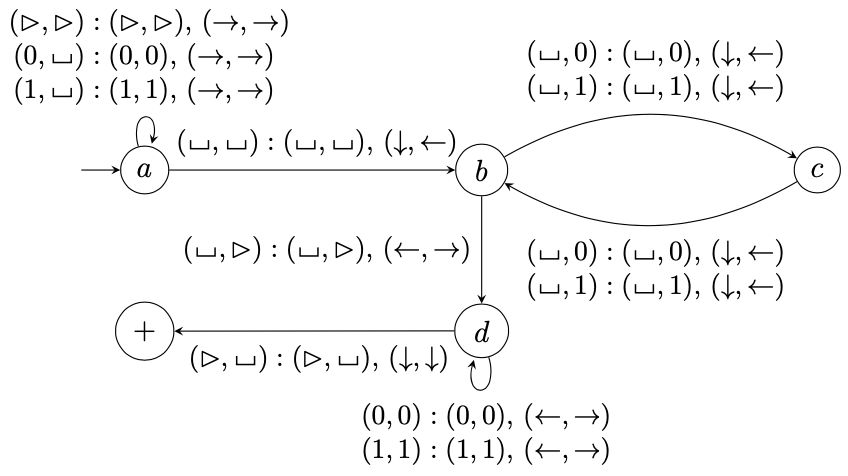
\includegraphics[width=0.8 \columnwidth]{images/Screen Shot 2023-01-13 at 13.03.05.png}
\subsubsection{Transition Functions}
\begin{tabular}{c c}
    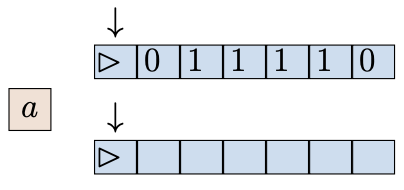
\includegraphics[width=0.4\columnwidth]{images/Screen Shot 2023-01-13 at 13.13.05.png} &  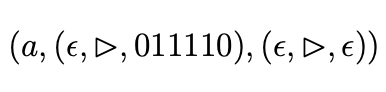
\includegraphics[width=0.4\columnwidth]{images/Screen Shot 2023-01-13 at 13.13.11.png}\\

\end{tabular}
The starting state is a. The first tuple specifies that nothing is to the left of the first tape head, that the first tape head is on the starting symbol, and that the input is to the right of the tape head.
\subsubsection{Robustness}

\begin{theorem}
For each multi-tape TM $M$ $\exists$ a 1-tape TM $M'$. Furthermore $M'$ halts for exactly the same inputs as $M$
\end{theorem}

\subsection{Church-Turing Thesis}
\textit{The class of functions computable by Turing machines encompasses all intuitively computable functions}. It is \textbf{not} provable.

\subsection{Decidability \& Computability}

\begin{definition}
     (Decidable)
     A set $L \subseteq \Sigma^*$ is called decidable if $\exists$ a TM $M$ which decides L.
\end{definition}

\hl{A TM that decides a language has to halt for all inputs over $\Sigma^*$, including those that are not in the language. As a consequence, if $L$ is decidable, then the complement $\Bar{L}$ of $L$ is also decidable.}

Decidability is concerned with yes-no questions, computability is about asking an openquestion demanding a result:
\begin{definition}
     (Computable, $\mathcal{R}$)
     A partial function $f: \Sigma^* \to \Sigma^*$ is called \textbf{computable} if it is Turing computable. $\mathcal{R}=$ the set of computable partial functions
\end{definition}

Note: Total functions are also partial functions

\subsubsection{Algorithmic Problems vs. Languages \& Functions}
How can "real" algorithmic problems be expressed by such sets or functions?

\textit{Encodings} All kinds of structures can be encoded by 0-1 strings.

\textit{Languages}
Algorithmic decision problems correspond to languages.

\section{Undecidable Problems (1)}

\subsection{"Hello, World!" Problems}

\subsubsection{Autom. Verification of General Programs}
\begin{definition}
     (Verification Problem)\\
     Input: Program P, property E
     Question: Does P feature property E?
\end{definition}

\begin{theorem*}
(Fermat's Theorem [Wiles 95])\\
$x^n+y^n=z^n$ has no integer solution for $x,y,z \in \mathbb{N}$ and $n \geq 3$
\end{theorem*}

\begin{corollary*}
This example program is not a "Hello, World!" program.
\end{corollary*}

There is no simple trick to avoid having to test infinitely many combinations.

\begin{definition}
     ("Hello, World!" Problem)\\ We denote a program for the “Hello, World!” problem as a “Hello, World!” tester. This tester will take a program P as input, and output “yes” if P is a “Hello, World!” program, and “no” otherwise.\\
     \textbf{Input:} Program P\\
     \textbf{Question:} Is P a "Hello, World!" program?
\end{definition}

\subsubsection{Tester}

\begin{theorem*}
     No "Hello, World!" testers exist
\end{theorem*}

\begin{definition}
     (“Hello, World!” Probl. with Input)\\
     \textbf{Input}: Program P, input I\\
\textbf{Question}: Does P return “hello, world” for the input I?
\end{definition}

\textit{"Proof by Contradiction": "Hello World!" Tester theorem.} Notation: Problem $P$, input $I$

Assume $\exists$ a tester $T$ 

\begin{center}
    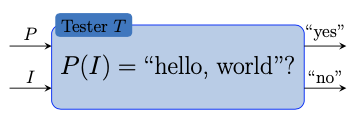
\includegraphics[width=0.55\columnwidth]{images/Screen Shot 2022-12-29 at 14.11.11.png}
\end{center}
 We construct a program $S$ with input $P'$ as follows: \begin{enumerate}
     \item Execute $T$ with inputs $P'$ (for $P$) and $P'$ (for $I$). We input $P'$ as both the program and input. $P'(P')$ 
     \item Return: \begin{itemize}
         \item "yes" if $T$ returns the outptut "yes"
         \item "hello, world", if $T$ returns output "no"
         \begin{center}
             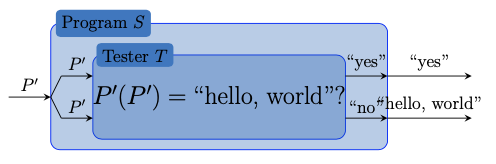
\includegraphics[width=0.7 \columnwidth]{images/Screen Shot 2022-12-29 at 14.16.42.png}
         \end{center}
     \end{itemize}
     We now consider $S$ run with input $S$:
     \begin{center}
             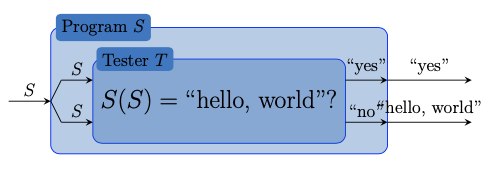
\includegraphics[width=0.7 \columnwidth]{images/Screen Shot 2022-12-29 at 14.19.19.png}
         \end{center}
 \end{enumerate}
 Both possible outputs lead to a contradiction of the assumption that $T$ is a tester for the "Hello, World!" problem with input. 

 We will show using a reduction that $\nexists$ a tester for the "hello world" problem without input. 
 
\subsection{First undecidable Problem}

Proof is similar to the proof that $\nexists$ program for solving the "hello, world!" problem.

\begin{definition}
     (TM-Diag)\\
     Input: Turing machine M\\ Question: Does M accept the input enc(M)
\end{definition}
 Can also be defined as language: \textsc{TM-Diag} = \{enc($M$) $|$ $M$ accepts the input enc($M$)\}
\begin{theorem}
{\sc{TM-Diag}} is not decidable
\end{theorem}

\paragraph{Diagonalization}
Enumerate all strings over $\Sigma^*$ with $\Sigma=\{0,1\}$, thus an enumeration of all Turing machines.

Consider the acceptance and termination behavior of $M_i$ for the input $v_j$ $\forall$ combos of $i$ and $j$.
Assume $\exists$ TM $M$ that decides \textsc{TM-Diag}.

%\begin{center}
%\includegraphics[width=0.5\columnwidth]{images/Screen Shot 2022-12-29 at 14.37.57.png}
%\end{center}
We modify $M$ to $M'$ by inverting the accepting behavior.

\begin{center}
\includegraphics[width=0.5\columnwidth]{images/Screen Shot 2022-12-29 at 14.39.55.png}
\end{center}

Now, there must exist $M_l=M'$ because we enumerated all TMs. Then it should hold:

\begin{tabular}{l l}
     & $M_l$ accepts $v_l$\\ 
     $\iff$ & $M'$ accepts $v_l$ \\
     $\iff$ & $M$ rejects $v_l$ 
\end{tabular}

This is a contradiction because we started by stating that $M_l$ accepts $v_l$. Thus \textsc{TM-Diag} is not decidable. 


\subsection{\hl{Reductions}}
\hl{Problem A reduces to problem B iff a solver for B can be used to solve problem A.

If $A$ reduces to $B$ and $B$ is "solvable" then A is "solvable"

If $A$ reduces to $B$ and $A$ is "unsolvable" then B is "unsolvable"}

\begin{definition}
     (Reduction). Let L, $L'  \in \Sigma^*$. A total computable function $F= \Sigma^* \to \Sigma^*$ is called a \textbf{reduction} from L to $L^'$ if $\forall x \in \Sigma^*: x \in L \implies f(x) \in L^'$
\end{definition}

\begin{definition}
     (Reducible). Let L, $L' \in \Sigma^*$ L is called \textbf{reducible} to $L'$ if  $\exists$ a reduction from L to $L'$. The notation to indicate this is $L \leq L'$
\end{definition}

\paragraph{Reductions as functions}
 %A reduction is essentially a function that maps the inputs and the outputs of each problem to the other problem.

 A reduction from $A$ to $B$ is a function\\ \hl{$f:\Sigma_1^* \to \Sigma_2^*$} such that:

 %$f(\mathcal{A})=(G_\mathcal{A},s,t)$ where $G_\mathcal{A}$ is the graph corresponding to automaton $\mathcal{A}$ and $s$ and $t$ are the initial and final node, respectively. Additionally: \begin{itemize}
     %\item $G_\mathcal{A}=(V_\mathcal{A},E_\mathcal{A})$, where $V_\mathcal{A}$ are the nodes and $E_\mathcal{A}$ are the edges
     %\item $V_\mathcal{A}=Q \cup \{s,t\}$  The graph will have a node for each state of the automaton, in
%addition to the initial and final nodes.
%\item $E_\mathcal{A}=\{(s,q_0)\} \cup \{(q,t)|q \in F\} \cup \{(q,q')| \delta (q, \sigma)= q', \sigma \in \Sigma\}$
 %\end{itemize} 
 
%\paragraph{Requirements} 
\begin{enumerate}
    \item $f$ is \textbf{\hl{total}} (defined for the entire domain)
    \item $f$ is \textbf{\hl{computable}} (in finitely many steps)
    \item \hl{$x \in L \iff f(x) \in L'$}
\end{enumerate}


\subsubsection{Reductions \& undecidable problems}

Reductions can prove that a decision problem $A'$ is undecidable. It is sufficient to show that a known undecidable problem $A$ is reducible to $A'$.

\subsubsection{\textsc{CFG-Intersection} \& \textsc{PCP}}

\begin{theorem}
    \textsc{PCP} $\leq$ \textsc{CFG-Intersection}
\end{theorem}
\subsection{Further undecidable Problems}
\begin{theorem}
    \textsc{TM-Halt} is not decidable
\end{theorem}
\textit{Proof Sketch} Show that \textsc{TM-Diag} $\leq$ \textsc{TM-Halt}.

\subsubsection{Undecidability of $\textsc{TM-Halt}$ \& $\textsc{TM-e-Halt}$}

\begin{tabular}{l l}
     \sc{TM-Halt} & \textit{Does M halt for the input x?} \\
     \sc{TM-e-Halt} & \textit{Does M halt for the input $\epsilon$?} \\
     \sc{TM-Diag} & \textit{Does M accept the input enc(M)?}
\end{tabular}

\section{Undecidable Problems (2)}
\subsection{Complements of Decidable Languages}
\begin{lemma} \hl{L is decidable $\implies$ $\Bar{L}$ is decidable} \\
$\Bar{L}$ undecidable $\implies$ L is undecidable
\end{lemma}
\subsection{\hl{Rice's Theorem}}

Any non-trivial semantic property of algorithms is undecidable.

\begin{theorem}
    \text{(Rice 53)} Let S be a set of computable partial functions with $\emptyset \neq S \neq \mathcal{R}$. Then \textsc{TM-Func(S)} is undecidable.
\end{theorem}



\paragraph{Proof}

\begin{enumerate}
    \item Define $S$ the subset of computable functions that have the property we want to check \hl{e.g.} $S=\{f \in \mathcal{R} | \forall x, \text{ it holds } f(x)=\bot \lor f(x)\neq 101\}$
    \item Show that $S\neq \emptyset$ and $S\neq \mathcal{R}$ holds by giving an example.
\end{enumerate}
\subsection{From SPCP to PCP}

\subsection{Undecid. Grammar Problems}

\begin{tabular}{l l}
     \sc{CFG-Intersection} & \textit{Is $L(G_1)\cap L(G_2)= \emptyset$?} \\
     \sc{CFG-Unamb} & \textit{Is G  unambiguous?}\\
     \sc{CFGEqui} & \textit{Is $L(G_1) = L(G_2)$?}\\
     \sc{CFGRegEqui} & \textit{Is $L(G_1) = L(\alpha)$?}\\
     \sc{CFGAll} & \textit{Is $L(G) = \Sigma^*$?}\\
     \sc{CFGCont} & \textit{Is $L(G_1) \subseteq L(G_2)$?}\\
\end{tabular}
$G$: Context-free grammar \
    $\alpha$: Reg. Expression
\section{Variants, Restrictions \& Extensions}

\subsection{Universal Turing Machines}
A universal TM $U$ takes as input a TM $M$, and can then simulate $M$.

\begin{center}
    \includegraphics[width=0.6\columnwidth]{images/Screen Shot 2022-12-29 at 15.56.29.png}
\end{center}
$U$ takes as input the machine $M$ and $x$, which is the input to $M$. It computes $f_M(x)$
\paragraph{Binary Encoding for Turing Machines} A standardisation of the encoding of TM.

\begin{center}
 \includegraphics[width=0.8\columnwidth]{images/Screen Shot 2022-12-29 at 16.01.33.png}   
\end{center}
\begin{tabular}{l l}
    states($q$) & enc($q$)=$0^{\text{num($q$)}}1$ \\
    symbols ($\sigma$) & enc($\sigma$)=$0^{\text{num($\sigma$)}}1$ \\ 
    directions ($d$) & enc($d$)=$0^{\text{num($d$)}}1$\\
\end{tabular}

transitions $\delta(q,\sigma)=(q#,\sigma', d)$: \\ enc($q, \sigma)=1$  enc($q$) enc($\sigma$) enc($q'$) enc($\sigma'$) enc($d$)

enc($M$) = concatenation of the strings enc($q, \sigma$)

1 serves as
a “stopping” symbol indicating the end of the encoding.

Assigning to eacht 0-1 string $w$ a TM $M_w$:
\begin{itemize}
    \item The TM $M$ with enc($M$)=$w$, if $\exists$ such a TM $M$
    \item TM $M_-$ which immediately switches to rejecting state by reading left border symbol $\rhd$, otherwise
\end{itemize}

input $x=x_1 ... x_m$ is encoded by enc($x$) = enc($x_1$) ... enc($x_m$)

For $y = enc(x)$, we write $x=enc^{-1}(y)$

In a sense, $enc^{-1}(y)$ is a “decoding” function that transforms the encoding back to the original TM.

\paragraph{Existence of the Universal Turing Machine}

\begin{definition}
    (Universal Turing Machine).  TM U is a universal Turing machine if for 0-1-strings w and x the following conditions are satisfied: \begin{itemize}
        \item $M_w$ accepts input enc$^{-1}(x) \implies$ U accepts input w\#x
        \item $M_w$ rejects input enc$^{-1}(x) \implies$ U rejects input w\#x
        \item $M_w$ doesn't halt for input enc$^{-1}(x) \implies$ U doesn't halt for input w\#x
    \end{itemize}
\end{definition}

\begin{center}
    \includegraphics[width=0.5\columnwidth]{images/Screen Shot 2022-12-29 at 16.36.30.png}
\end{center}

\begin{theorem}
    $\exists$ a universal Turing machine 
\end{theorem}

\subsection{Semi-Decidability}
%Not every Turing machine $M$ decides a language, since it may not halt for every input. Nonetheless, every machine will halt for some set of strings (which may be empty). We call that set L($M$). $M$ will halt and accept for each word in L($M$), and it can either halt and reject or never halt for words not in L($M$). We call the set L(M) \textbf{semi-decidable}. In a sense, we can “decide” the yes- part, but not the no-part.

\begin{definition}
    \hl{(Semi-decidability)} A set $L \subseteq \Sigma^*$ is called semi-decidable if $\exists$ a TM M with L=L(M)
\end{definition}

\begin{itemize}
    \item \hl{Halts and accepts for all “yes” inputs.}
    \item \hl{Does not halt for or rejects all other inputs.}
\end{itemize}
%It's ok if the TM doesn't halt for some inputs $x \notin L$. 

Every decidable language is also semi-decidable.

\subsubsection{ Examples of Semi-Decidable Languages}
\textsc{CFG-Intersection} \textit{Is L($G_1) \cap L(G_2)\neq \emptyset$?}
One can use the \textsc{CYK} algo to test whether $w \in L(G_1)$ \& $w \in L(G_2)$

Further exmaples: \textsc{TM-Diag, TM-Halt, PCP,...}

\subsubsection{ Decidability \& Semi-Decidability}

\begin{lemma}
    \hl{Let L be a language. Then it holds:
    L decidable $\iff$ L and $\Bar{L}$ semi-decidable}
\end{lemma}
\subsubsection{Non Semi-Decidable Problems}
\hl{Lemma 14.2 can be used to verify that a language is not semi-decidable.}

\begin{definition}
    \textsc{(CFG-Disjunct)}\\ Is L($G_1) \cap L(G_2)= \emptyset$?
\end{definition}

\begin{lemma}
    \textsc{CFG-Disjunct} is not semi-decidable.
\end{lemma}

\subsubsection{Semi-Decid. vs. Recursively Enumerable}

\begin{definition}
    (Recursively Enumerable) A langueage L is recursively enumerable if $\exists$ a 2-tape TM M that progressively writes all element of L onto its second tape.
\end{definition}

\begin{lemma}
    L is recursively enumerable $\iff$ L is semi-decidable
\end{lemma}

\subsubsection{Decidability vs. Computability}

\begin{definition}
    (Characteristic Function) Let L be a language. The characteristic function of L, $\chi_L: \Sigma^* \to \{0,1\}$, is defined by: \\
    $\chi_L  (w) = \begin{cases}
        1 & w \in L \\
        0 & w \notin L
    \end{cases}$\\
The partial characteristic function of L, $\chi'_L: \Sigma^* \to \{0,1\}$, is defined by: \\
    $\chi_L  (w) = \begin{cases}
        1 & w \in L \\
        \bot & w \notin L
    \end{cases}$
\end{definition}

\begin{lemma}
    L decidable $\iff \chi_L$ computable\\
    L semi-decidable $\iff \chi'_L$ computable
\end{lemma}
\section{Polynomial Time}
\begin{definition}
\textsc{MinSpanningTreeO}\\
    Input: Undirected Graph G=(V,E), weighting function l:E$\to \mathcal{N}$\\
    Question: Spanning tree T $\subseteq E$ of G with minimal total weight
\end{definition}
\subsection{Prim's Algorithm}
To calculate min spanning tree. Start at any node. Always choose the adjacent edge with the least weight and add it to the graph.

\subsubsection{Comft. Bridge Building \& Min Cycles}
\begin{definition}
\textsc{MinCycleO}\\
    Input: Undirected Graph G=(V,E), distance function l:E$\to \mathcal{N}$\\
    Desired output: Cycle K $\subseteq E$ through all nodes with minimal total weight. If $\nexists$ such a cycle, the value should be $\infty$.
\end{definition}

\subsubsection{Minimal Cycles: Algo}
Best algo has a complexty of $> n! $
\subsection{Comp. Cost \& Compl. Theory}

\subsubsection{Complexity}
In this lecture measured in runtime 
\subsubsection{Asymptotic Worst-case Complexity}
complexity: function of the input size.

\subsubsection{Purpose of Complexity Theory}
Problems are categorized according to their principal algorithmic difficulty into "efficiently solvable" and "not efficiently solvable"

\paragraph{Complexity classes}
\begin{enumerate}
    \item Mode of computation (deterministic, probabilistic, parallel etc.)
    \item Type of considered resource (runtime, memory space...)
    \item Growth behavior (log, exp..)
\end{enumerate}

\paragraph{$P \neq NP$?}
In polynoml time, can more problems be solved nondeterministically (\textbf{$NP$}) than determin. (\textbf{$P$})

\subsection{Efficiently solvable Decision Problems}

The runtime is quantified as the number of steps of a computation. A single step composed of several operations (reading tape, change state..)

\begin{definition}
    (Runtime of TMs) If $K_0 \vdash_M K_1 \vdash_M K_2 \dots \vdash_M K_m $ is a computation of a TM M for the input x and $K_m$ a halting configuration, then we define:\\ 
        $t_M(x)=m:$ runtime of $M$ for the input $x$\\
        If $\nexists$ such finite sequence: $t_M(x)=\bot$

\end{definition}


\begin{definition}
    (Input size): len(input string)
\end{definition}

\begin{definition}
    (Time Bound). A function $T: \mathcal{N}\to \mathbb{R}$ is called a time bound for a TM M if $\exists$ an $n_0 \in \mathcal{N}$ such that $\forall x \in \Sigma^*$ with $|x|>n_0:t_M(x)\leq T(|x|)$
\end{definition}

\begin{definition}
    \textsc{(TIME $(T)$, P)}.For $T: \mathcal{N} \to \mathbb{R}$ let \textsc{TIME} (T) be the set of all languages L for which $\exists$ a k-tape TM M with time bound T such that L=L(M)\\
    P= $\underset{\text{p polynomial}}{\bigcup}$ TIME(p)
\end{definition}


%\subsubsection{P $\equiv$ Efficiently Solvable Problems?}
%Objections:
%\begin{itemize}
%    \item Polynomials with large exponents are far from efficient
 %   \item Worst-case is unsuitable, the average case would be much more interesting
 %   \item Decision problems (languages) are too restricted
%\end{itemize}
\stepcounter{subsubsection}

\subsubsection{Problems Not solvable in Polynomial Time}
\begin{definition}
    \text{(EXPTIME)}: $\underset{\text{p polynomial}}{\bigcup}$ TIME($2^p)$
\end{definition}

\subsubsection{Polynomial Time Bounds. $n^k$}
Simplified expression for complexity

\subsection{Optimization Problems vs.\\ Decision Problems}
Optimisation problems can be expressed as decision problems.

\subsubsection{Travelling Salesperson Probl.}
Shortest round trip through a set of cities visiting each city exactly once.

\begin{definition}
    (TSP - decision problem). \\Input: Distance function d, target value $k \in \mathcal{N}$\\
    Question: $\exists$ TSP route f for d with dist(f) $\leq$ k?
\end{definition}

\begin{definition}
    (TSPO - optimisation problem). \\Input: Distance function d\\
    Desired output: TSP route f for d with minimal total distance
\end{definition}

\begin{definition}
    (TSPV - value problem). \\Input: Distance function d\\
    Desired output: Distance dist(f) of a TSP route f for d with minimal total distance
\end{definition}
\textit{Proof Sketch.} Let $d$ be a distance function for TSPV with $n$ cities. It is then possible to use a binary search algorithm to find the value of the minimal distance. The TSP optimization problem can thus be reduced in polynomial time to the TSP decision problem.

\begin{lemma}
    If TSP is solvable in polynomial time, then TSPV is as well. If TSPV is solvable in polynomial time, then TSPO is as well.
   \end{lemma}
 
\section{NP-Completeness}

\subsection{Examples of Difficult Computational Problems}


%\subsubsection{Knapsack}
\stepcounter{subsubsection}
\stepcounter{subsubsection}
\begin{definition}
    \textsc{(Knapsack)}.\\ Input: Weight limit W, desired Value V, m objects with values v nd weights w. \\
    Question: Is there $I \subset \{1, \dots , m\}$ such that $\Sigma_{i \in I} v_i\geq V$ and $\Sigma_{i \in I} w_i\geq W$?
\end{definition}

%\subsubsection{Graph Coloring}

\begin{definition}
    \textsc{(Col)}. \\
    Input: Undirected graph G, number k\\
    Question: Can the nodes of G be properly colored with k colors, i.e. such that the nodes connected by edges have different colors?
\end{definition}
\subsubsection{Graph Theory Refresher}

    A \textbf{walk} is a sequence of consecutive edges. Nodes and edges can be repeated.

A \textbf{path} is a walk that does not go through  the same node more than once. Note that a path can start and finish in the same node.

    A \textbf{closed walk} is a  walk that starts and ends in the same node.

    
%\subsubsection{Euler Cycles}
\stepcounter{subsubsection}

\begin{definition}
\textsc{(EulerCycle)}\\
Input: Undirected graph G\\
Question: $\exists$ a closed walk which visits \textbf{each edge} exactly once?
\end{definition}

\begin{theorem*}
    A connected graph G has an Euler cycle iff each node has even degree (number of adjacent nodes).
\end{theorem*}

%\subsubsection{Hamiltonian Cycles}
\stepcounter{subsubsection}
\begin{definition}
\textsc{(HamiltonianCycle)}\\
Input: Undirected graph G\\
Question: $\exists$ a closed walk which visits \textbf{each node} exactly once?
\end{definition}

\subsubsection{Clique Problem}

\begin{definition}
    (Clique). Two nodes u, v of an undirected graph G = (V, E) are called adjacent if (u, v) $\in$ E. A k-clique is a set C of k nodes which are pairwise adjacent.
\end{definition}

\begin{definition}
    \textsc{(Clique)}. \\
    Input: Graph G = (V,E), number k\\
    Question: $\exists$ clique G with k nodes?
\end{definition}

\subsubsection{Prop. Logic Satisfiability (SAT, 3-SAT)}

\begin{definition}
    (Propositional Logic Formula). Let $x_1, x_2, x_3, \dots$ be variables \begin{itemize}
        \item Each $x_i$ is a propositional logic formula
        \item If $\phi$ is such a formula, then $\lnot \phi$ is as well.
        \item If $\phi_1, \phi_2$ are such formulas, then $\phi_1 \land \phi_2$ and $\phi_1 \lor \phi_2$ are too.
        \item A truth assignment $\alpha: \{x_1, x_2, ...\} \to \{0,1\}$ assigns 0 or 1 to each variable.
        \item $\alpha \models \phi$ ("$\alpha$ models $\phi"$): The formula $\phi$ evaluates to q under the assignment $\alpha$
        \item A formula $\phi$ is satisfiable if $\exists \alpha$ with $\alpha \models \phi$
    \end{itemize}
\end{definition}

\subsection{\hl{NP}}
Stands for non-deterministically polynomial. It refers to problems for which checking the correctness of a proof candidate takes polynomial time. 

Known algo $\in P$: \textsc{EulerCycle}; \textsc{MinSpanTreeO}

No known algo $\in P$: \textsc{TSP; HamiltonianCycle; SAT; Col; Knapsack; 3-SAT, Clique}

The NP have in common that they can be solved by "brute force".

\paragraph{\hl{Properties}}
\begin{enumerate}
    \item They have a search space of proof candidates.
    \item The proof candidates are polynomially large in the input.
    \item Each proof candidate can be checked in polynomial time.
\end{enumerate}

(note that we do not need to come up with the proof candidate)

For all these problems, there exists for each input a set of \textbf{proof candidates} e.g. for \textsc{Col}: all colorings with $k$ colors.
%More examples?

\subsubsection{Formalizing the definition of NP}
\begin{definition}
    (Non-deterministically Accepting/Deciding). Let $\Sigma=\{0,1\}$ 
    \begin{itemize}
        \item M \textbf{non-deterministically accepts} a string $w \in \Sigma^*$ if $\exists$ string $y \in \Sigma^*$ s.t. M (deterministically accepts the input (w,y)
        \item The string y is called the extra input (proof candidate)
        \item M \textbf{non-deterministically decides} a language $L \subseteq \Sigma^*$ if $\forall$ strings w $\in \Sigma^*$:\begin{itemize}
            \item $w \in L \Rightarrow$M accepts w non-deterministically\\
            \* $\exists$ y s.t. M accepts (w,y)
            \item $w \notin L:$ M does not accept w non-deterministically 
            $\Rightarrow \nexists$ y s.t. M accepts (w,y)
        \end{itemize}
    \end{itemize}
\end{definition}

We denote the computation time of $M$ for the input $(w,y)$ by $t_M(w,y)$

\begin{definition}
    \textsc{(NTIME($T$),NP)} Let $\Sigma=\{0,1\}, T:\mathcal{N}\to \mathbb{R}$\begin{itemize}
        \item \textsc{(NTIME($T$)}= class of all $L\subseteq\Sigma^*$  $\exists$ TM M which decides L non-deterministically s.t. $\forall$ w,y, $\in \Sigma^*:t_M(w,y) \leq T(|w|)$
        \item $NP=\underset{\text{p polynomial}}{\bigcup}NTIME(p)$
    \end{itemize}
\end{definition}
%\subsubsection{Notes on NP}
\stepcounter{subsubsection}
%\subsubsection{P vs. NP}
%For a problem to be in NP, it suffices that there exists an algorithm which efficiently checks if a proof candidate is a proof.

\begin{proposition}
    $P \subseteq NP \subseteq EXPTIME$
\end{proposition}

\subsection{NP-Completeness}
\subsubsection{Similarity of Difficult Decision Problems} They can all be linked together by polynomial reductions. This means that either they can all be solved in polynomial time or none of them can.

\subsubsection{Polynomial Reductions}
\begin{definition}
    (\hl{Polynomial Reduction} $\leq_p$). A \hl{total} function f from L to L' is a polynomial reduction if: \begin{enumerate}
        \item f is a reduction from L to L', i.e. $\forall \ w \in \Sigma^*:$ \hl{$w \in L \iff f(w) \in L'$}
        \item f is \hl{computable in polynomial time}
    \end{enumerate}
    L is polynomially reducible: $L \leq_p L'$
\end{definition}

\subsubsection{NP-hard Problems}
\begin{definition}
    \hl{(NP-hard)}. A language L is called NP-hard if \hl{$\forall \ L' \in NP: L' \leq_p L$}
\end{definition}

A problem is NP-hard if it is at least as hard as other problems in NP.

\begin{proposition}
    \textsc{TM-Halt} is NP-hard
\end{proposition}

Any language $L \in NP$ can be reduced in polynomial time to \textsc{TM-Halt}

%\textit{Proof Sketch.}\begin{itemize}
%    \item Let $L \in NP \implies L \in EXPTIME$
 %   \item ...
%\end{itemize}

\begin{definition}
    \hl{(NP-complete)}. A langueage L is called NP-complete \hl{if L is NP-hard and $L \in NP$}
\end{definition}

\begin{proposition}
    Let $L,L'\subseteq \Sigma^*$ with $L\leq_p L'$:\begin{enumerate}
        \item $L' \in P \implies L \in P$
        \item $L' \in NP \implies L \in NP$
    \end{enumerate}
\end{proposition}

\begin{corollary}
    Let $L,L'\subseteq \Sigma^*$ and let $L\leq_p L'$. If $L \notin P \implies L' \notin P$
\end{corollary}

\stepcounter{theorem}\stepcounter{theorem}\stepcounter{theorem}\stepcounter{theorem}

\begin{theorem}
    Let L be an NP-complete problem. \begin{itemize}
        \item If $L \in P \implies P = NP$
        \item If $L \notin P \implies P \neq NP$
    \end{itemize}
\end{theorem}
\subsection{Cook-Levin Theorem}
Prove that at least one problem is NP-complete. 
\begin{theorem}
    (cook 71, Levin 73). SAT is NP-complete.
\end{theorem}
\section{NP-Complete Problems}
Use polynomial reductions to show that other problems are also NP-complete.

\subsection{Polynomial Reductions}
\begin{center}
    \includegraphics[width=0.8\columnwidth]{images/Screen Shot 2023-01-05 at 18.04.01.png}
\end{center}

%\begin{lemma}
 %   Let $L_1, L_2, L_3 \subseteq \Sigma^*$ be languages. If $L_1 \leq_p L_2$ and $L_2 \leq_p L_3$, then also $L_1 \leq_p L_3$
%\end{lemma}

%\begin{lemma}
    %If L' is NP-hard and L' $\leq_p L$ holds, then L is also NP-hard.
%\end{lemma}
%\subsubsection{Reductions and NP-Completeness}

%\subsubsection{3-SAT}
%\begin{proposition}
   % SAT $\leq_p$ 3-SAT
%\end{proposition}

%\subsubsection{Clique Problem}

%\subsubsection{3-Colorability}

%\subsubsection{Hamiltonian Cycles and TSP}

%\subsection{Subset Sums and the Knapsack Problem}
%\begin{definition}
    %\textsc{SubsetSum}\\Input: Set S of natural numbers and  target number k\\Question:  $\exists \ T\subseteq S$ with $\Sigma_{a\in T}\ a=k$?
%\end{definition}
%\subsubsection{SubsetSum $\leq_p$ Knapsack}

%\subsubsection{Overall Results and Remarks}
\begin{theorem}
    The following problems are NP-complete: \textsc{3-SAT; 3-Col; Clique; HamiltonianCycle; TSP; SubsetSum; Knapsack}
\end{theorem}

%\subsubsection{Pseudo-polynomial vs. strong NP-completeness}

\paragraph{Classify a language at first sight}
Look at the exponents of the different alphabets. Is there any relation between the different exponents?
\begin{itemize}
    \item \textbf{No}. The language is \textbf{regular} and \textbf{context-free}. EG: $L=a^mb^n \ | \ m,n\geq 0$
    \item \textbf{Yes, one} eg: $L=a^mb^n \ | \ m > n, m \neq n $ These languages are not regular, but are context-free and accepted by a PDA.
    \item \textbf{Yes, multiple} not regular and not context-free
\end{itemize} 
\end{multicols*}
\end{document}